\documentclass{report}

%%%%%%%%%%%%%%%%%%%%%%%%%%%%%%%%%
% PACKAGE IMPORTS
%%%%%%%%%%%%%%%%%%%%%%%%%%%%%%%%%


\usepackage[tmargin=2cm,rmargin=1in,lmargin=1in,margin=0.85in,bmargin=2cm,footskip=.2in]{geometry}
\usepackage{amsmath,amsfonts,amsthm,amssymb,mathtools}
\usepackage[varbb]{newpxmath}
\usepackage{xfrac}
\usepackage[makeroom]{cancel}
\usepackage{mathtools}
\usepackage{bookmark}
\usepackage{enumitem}
\usepackage{hyperref,theoremref}
\hypersetup{
	pdftitle={Assignment},
	colorlinks=true, linkcolor=doc!90,
	bookmarksnumbered=true,
	bookmarksopen=true
}
\usepackage[most,many,breakable]{tcolorbox}
\usepackage{xcolor}
\usepackage{varwidth}
\usepackage{varwidth}
\usepackage{etoolbox}
%\usepackage{authblk}
\usepackage{nameref}
\usepackage{multicol,array}
\usepackage{tikz-cd}
\usepackage[ruled,vlined,linesnumbered]{algorithm2e}
\usepackage{comment} % enables the use of multi-line comments (\ifx \fi) 
\usepackage{import}
\usepackage{xifthen}
\usepackage{pdfpages}
\usepackage{transparent}
\usepackage{youngtab}

\newcommand\mycommfont[1]{\footnotesize\ttfamily\textcolor{blue}{#1}}
\SetCommentSty{mycommfont}
\newcommand{\incfig}[1]{%
    \def\svgwidth{\columnwidth}
    \import{./figures/}{#1.pdf_tex}
}

\usepackage{tikzsymbols}
\renewcommand\qedsymbol{$\Laughey$}


%\usepackage{import}
%\usepackage{xifthen}
%\usepackage{pdfpages}
%\usepackage{transparent}


%%%%%%%%%%%%%%%%%%%%%%%%%%%%%%
% SELF MADE COLORS
%%%%%%%%%%%%%%%%%%%%%%%%%%%%%%



\definecolor{myg}{RGB}{56, 140, 70}
\definecolor{myb}{RGB}{45, 111, 177}
\definecolor{myr}{RGB}{199, 68, 64}
\definecolor{mytheorembg}{HTML}{F2F2F9}
\definecolor{mytheoremfr}{HTML}{00007B}
\definecolor{mylenmabg}{HTML}{FFFAF8}
\definecolor{mylenmafr}{HTML}{983b0f}
\definecolor{mypropbg}{HTML}{f2fbfc}
\definecolor{mypropfr}{HTML}{191971}
\definecolor{myexamplebg}{HTML}{F2FBF8}
\definecolor{myexamplefr}{HTML}{88D6D1}
\definecolor{myexampleti}{HTML}{2A7F7F}
\definecolor{mydefinitbg}{HTML}{E5E5FF}
\definecolor{mydefinitfr}{HTML}{3F3FA3}
\definecolor{notesgreen}{RGB}{0,162,0}
\definecolor{myp}{RGB}{197, 92, 212}
\definecolor{mygr}{HTML}{2C3338}
\definecolor{myred}{RGB}{127,0,0}
\definecolor{myyellow}{RGB}{169,121,69}
\definecolor{myexercisebg}{HTML}{F2FBF8}
\definecolor{myexercisefg}{HTML}{88D6D1}


%%%%%%%%%%%%%%%%%%%%%%%%%%%%
% TCOLORBOX SETUPS
%%%%%%%%%%%%%%%%%%%%%%%%%%%%

\setlength{\parindent}{1cm}
%================================
% THEOREM BOX
%================================

\tcbuselibrary{theorems,skins,hooks}
\newtcbtheorem[number within=section]{Theorem}{Theorem}
{%
	enhanced,
	breakable,
	colback = mytheorembg,
	frame hidden,
	boxrule = 0sp,
	borderline west = {2pt}{0pt}{mytheoremfr},
	sharp corners,
	detach title,
	before upper = \tcbtitle\par\smallskip,
	coltitle = mytheoremfr,
	fonttitle = \bfseries\sffamily,
	description font = \mdseries,
	separator sign none,
	segmentation style={solid, mytheoremfr},
}
{th}

\tcbuselibrary{theorems,skins,hooks}
\newtcbtheorem[number within=chapter]{theorem}{Theorem}
{%
	enhanced,
	breakable,
	colback = mytheorembg,
	frame hidden,
	boxrule = 0sp,
	borderline west = {2pt}{0pt}{mytheoremfr},
	sharp corners,
	detach title,
	before upper = \tcbtitle\par\smallskip,
	coltitle = mytheoremfr,
	fonttitle = \bfseries\sffamily,
	description font = \mdseries,
	separator sign none,
	segmentation style={solid, mytheoremfr},
}
{th}


\tcbuselibrary{theorems,skins,hooks}
\newtcolorbox{Theoremcon}
{%
	enhanced
	,breakable
	,colback = mytheorembg
	,frame hidden
	,boxrule = 0sp
	,borderline west = {2pt}{0pt}{mytheoremfr}
	,sharp corners
	,description font = \mdseries
	,separator sign none
}

%================================
% Corollery
%================================
\tcbuselibrary{theorems,skins,hooks}
\newtcbtheorem[number within=section]{Corollary}{Corollary}
{%
	enhanced
	,breakable
	,colback = myp!10
	,frame hidden
	,boxrule = 0sp
	,borderline west = {2pt}{0pt}{myp!85!black}
	,sharp corners
	,detach title
	,before upper = \tcbtitle\par\smallskip
	,coltitle = myp!85!black
	,fonttitle = \bfseries\sffamily
	,description font = \mdseries
	,separator sign none
	,segmentation style={solid, myp!85!black}
}
{th}
\tcbuselibrary{theorems,skins,hooks}
\newtcbtheorem[number within=chapter]{corollary}{Corollary}
{%
	enhanced
	,breakable
	,colback = myp!10
	,frame hidden
	,boxrule = 0sp
	,borderline west = {2pt}{0pt}{myp!85!black}
	,sharp corners
	,detach title
	,before upper = \tcbtitle\par\smallskip
	,coltitle = myp!85!black
	,fonttitle = \bfseries\sffamily
	,description font = \mdseries
	,separator sign none
	,segmentation style={solid, myp!85!black}
}
{th}


%================================
% LENMA
%================================

\tcbuselibrary{theorems,skins,hooks}
\newtcbtheorem[number within=section]{Lenma}{Lenma}
{%
	enhanced,
	breakable,
	colback = mylenmabg,
	frame hidden,
	boxrule = 0sp,
	borderline west = {2pt}{0pt}{mylenmafr},
	sharp corners,
	detach title,
	before upper = \tcbtitle\par\smallskip,
	coltitle = mylenmafr,
	fonttitle = \bfseries\sffamily,
	description font = \mdseries,
	separator sign none,
	segmentation style={solid, mylenmafr},
}
{th}

\tcbuselibrary{theorems,skins,hooks}
\newtcbtheorem[number within=chapter]{lenma}{Lenma}
{%
	enhanced,
	breakable,
	colback = mylenmabg,
	frame hidden,
	boxrule = 0sp,
	borderline west = {2pt}{0pt}{mylenmafr},
	sharp corners,
	detach title,
	before upper = \tcbtitle\par\smallskip,
	coltitle = mylenmafr,
	fonttitle = \bfseries\sffamily,
	description font = \mdseries,
	separator sign none,
	segmentation style={solid, mylenmafr},
}
{th}


%================================
% PROPOSITION
%================================

\tcbuselibrary{theorems,skins,hooks}
\newtcbtheorem[number within=section]{Prop}{Proposition}
{%
	enhanced,
	breakable,
	colback = mypropbg,
	frame hidden,
	boxrule = 0sp,
	borderline west = {2pt}{0pt}{mypropfr},
	sharp corners,
	detach title,
	before upper = \tcbtitle\par\smallskip,
	coltitle = mypropfr,
	fonttitle = \bfseries\sffamily,
	description font = \mdseries,
	separator sign none,
	segmentation style={solid, mypropfr},
}
{th}

\tcbuselibrary{theorems,skins,hooks}
\newtcbtheorem[number within=chapter]{prop}{Proposition}
{%
	enhanced,
	breakable,
	colback = mypropbg,
	frame hidden,
	boxrule = 0sp,
	borderline west = {2pt}{0pt}{mypropfr},
	sharp corners,
	detach title,
	before upper = \tcbtitle\par\smallskip,
	coltitle = mypropfr,
	fonttitle = \bfseries\sffamily,
	description font = \mdseries,
	separator sign none,
	segmentation style={solid, mypropfr},
}
{th}


%================================
% CLAIM
%================================

\tcbuselibrary{theorems,skins,hooks}
\newtcbtheorem[number within=section]{claim}{Claim}
{%
	enhanced
	,breakable
	,colback = myg!10
	,frame hidden
	,boxrule = 0sp
	,borderline west = {2pt}{0pt}{myg}
	,sharp corners
	,detach title
	,before upper = \tcbtitle\par\smallskip
	,coltitle = myg!85!black
	,fonttitle = \bfseries\sffamily
	,description font = \mdseries
	,separator sign none
	,segmentation style={solid, myg!85!black}
}
{th}



%================================
% Exercise
%================================

\tcbuselibrary{theorems,skins,hooks}
\newtcbtheorem[number within=section]{Exercise}{Exercise}
{%
	enhanced,
	breakable,
	colback = myexercisebg,
	frame hidden,
	boxrule = 0sp,
	borderline west = {2pt}{0pt}{myexercisefg},
	sharp corners,
	detach title,
	before upper = \tcbtitle\par\smallskip,
	coltitle = myexercisefg,
	fonttitle = \bfseries\sffamily,
	description font = \mdseries,
	separator sign none,
	segmentation style={solid, myexercisefg},
}
{th}

\tcbuselibrary{theorems,skins,hooks}
\newtcbtheorem[number within=chapter]{exercise}{Exercise}
{%
	enhanced,
	breakable,
	colback = myexercisebg,
	frame hidden,
	boxrule = 0sp,
	borderline west = {2pt}{0pt}{myexercisefg},
	sharp corners,
	detach title,
	before upper = \tcbtitle\par\smallskip,
	coltitle = myexercisefg,
	fonttitle = \bfseries\sffamily,
	description font = \mdseries,
	separator sign none,
	segmentation style={solid, myexercisefg},
}
{th}

%================================
% EXAMPLE BOX
%================================

\newtcbtheorem[number within=section]{Example}{Example}
{%
	colback = myexamplebg
	,breakable
	,colframe = myexamplefr
	,coltitle = myexampleti
	,boxrule = 1pt
	,sharp corners
	,detach title
	,before upper=\tcbtitle\par\smallskip
	,fonttitle = \bfseries
	,description font = \mdseries
	,separator sign none
	,description delimiters parenthesis
}
{ex}

\newtcbtheorem[number within=chapter]{example}{Example}
{%
	colback = myexamplebg
	,breakable
	,colframe = myexamplefr
	,coltitle = myexampleti
	,boxrule = 1pt
	,sharp corners
	,detach title
	,before upper=\tcbtitle\par\smallskip
	,fonttitle = \bfseries
	,description font = \mdseries
	,separator sign none
	,description delimiters parenthesis
}
{ex}

%================================
% DEFINITION BOX
%================================

\newtcbtheorem[number within=section]{Definition}{Definition}{enhanced,
	before skip=2mm,after skip=2mm, colback=red!5,colframe=red!80!black,boxrule=0.5mm,
	attach boxed title to top left={xshift=1cm,yshift*=1mm-\tcboxedtitleheight}, varwidth boxed title*=-3cm,
	boxed title style={frame code={
					\path[fill=tcbcolback]
					([yshift=-1mm,xshift=-1mm]frame.north west)
					arc[start angle=0,end angle=180,radius=1mm]
					([yshift=-1mm,xshift=1mm]frame.north east)
					arc[start angle=180,end angle=0,radius=1mm];
					\path[left color=tcbcolback!60!black,right color=tcbcolback!60!black,
						middle color=tcbcolback!80!black]
					([xshift=-2mm]frame.north west) -- ([xshift=2mm]frame.north east)
					[rounded corners=1mm]-- ([xshift=1mm,yshift=-1mm]frame.north east)
					-- (frame.south east) -- (frame.south west)
					-- ([xshift=-1mm,yshift=-1mm]frame.north west)
					[sharp corners]-- cycle;
				},interior engine=empty,
		},
	fonttitle=\bfseries,
	title={#2},#1}{def}
\newtcbtheorem[number within=chapter]{definition}{Definition}{enhanced,
	before skip=2mm,after skip=2mm, colback=red!5,colframe=red!80!black,boxrule=0.5mm,
	attach boxed title to top left={xshift=1cm,yshift*=1mm-\tcboxedtitleheight}, varwidth boxed title*=-3cm,
	boxed title style={frame code={
					\path[fill=tcbcolback]
					([yshift=-1mm,xshift=-1mm]frame.north west)
					arc[start angle=0,end angle=180,radius=1mm]
					([yshift=-1mm,xshift=1mm]frame.north east)
					arc[start angle=180,end angle=0,radius=1mm];
					\path[left color=tcbcolback!60!black,right color=tcbcolback!60!black,
						middle color=tcbcolback!80!black]
					([xshift=-2mm]frame.north west) -- ([xshift=2mm]frame.north east)
					[rounded corners=1mm]-- ([xshift=1mm,yshift=-1mm]frame.north east)
					-- (frame.south east) -- (frame.south west)
					-- ([xshift=-1mm,yshift=-1mm]frame.north west)
					[sharp corners]-- cycle;
				},interior engine=empty,
		},
	fonttitle=\bfseries,
	title={#2},#1}{def}



%================================
% Solution BOX
%================================

\makeatletter
\newtcbtheorem{question}{Question}{
	enhanced,
	% breakable,
	colback=white,
	% colframe=myb!80!black,
	% attach boxed title to top left={yshift*=-\tcboxedtitleheight},
	fonttitle=\bfseries,
	title={#2},
	% boxed title size=title,
	% boxed title style={%
	% 		sharp corners,
	% 		rounded corners=northwest,
	% 		colback=tcbcolframe,
	% 		boxrule=0pt,
	% 	},
	% underlay boxed title={%
	% 		\path[fill=tcbcolframe] (title.south west)--(title.south east)
	% 		to[out=0, in=180] ([xshift=5mm]title.east)--
	% 		(title.center-|frame.east)
	% 		[rounded corners=\kvtcb@arc] |-
	% 		(frame.north) -| cycle;
	% 	},
	#1
}{def}
\makeatother

%================================
% SOLUTION BOX
%================================

\makeatletter
\newtcolorbox{solution}{enhanced,
	breakable,
	colback=white,
	colframe=myg!80!black,
	attach boxed title to top left={yshift*=-\tcboxedtitleheight},
	title=Solution,
	boxed title size=title,
	boxed title style={%
			sharp corners,
			rounded corners=northwest,
			colback=tcbcolframe,
			boxrule=0pt,
		},
	underlay boxed title={%
			\path[fill=tcbcolframe] (title.south west)--(title.south east)
			to[out=0, in=180] ([xshift=5mm]title.east)--
			(title.center-|frame.east)
			[rounded corners=\kvtcb@arc] |-
			(frame.north) -| cycle;
		},
}
\makeatother

%================================
% Question BOX
%================================

\makeatletter
\newtcbtheorem{qstion}{Question}{
	% enhanced,
	% breakable,
	% colback=white,
	% colframe=mygr,
	% attach boxed title to top left={yshift*=-\tcboxedtitleheight},
	fonttitle=\bfseries,
	title={#2},
	% boxed title size=title,
	% boxed title style={%
	% 		sharp corners,
	% 		rounded corners=northwest,
	% 		colback=tcbcolframe,
	% 		boxrule=0pt,
	% 	},
	% underlay boxed title={%
	% 		\path[fill=tcbcolframe] (title.south west)--(title.south east)
	% 		to[out=0, in=180] ([xshift=5mm]title.east)--
	% 		(title.center-|frame.east)
	% 		[rounded corners=\kvtcb@arc] |-
	% 		(frame.north) -| cycle;
	% 	},
	#1
}{def}
\makeatother

\newtcbtheorem[number within=chapter]{wconc}{Wrong Concept}{
	breakable,
	enhanced,
	colback=white,
	colframe=myr,
	arc=0pt,
	outer arc=0pt,
	fonttitle=\bfseries\sffamily\large,
	colbacktitle=myr,
	attach boxed title to top left={},
	boxed title style={
			enhanced,
			skin=enhancedfirst jigsaw,
			arc=3pt,
			bottom=0pt,
			interior style={fill=myr}
		},
	#1
}{def}



%================================
% NOTE BOX
%================================

\usetikzlibrary{arrows,calc,shadows.blur}
\tcbuselibrary{skins}
\newtcolorbox{note}[1][]{%
	enhanced jigsaw,
	colback=gray!20!white,%
	colframe=gray!80!black,
	size=small,
	boxrule=1pt,
	title=\textbf{Note:-},
	halign title=flush center,
	coltitle=black,
	breakable,
	drop shadow=black!50!white,
	attach boxed title to top left={xshift=1cm,yshift=-\tcboxedtitleheight/2,yshifttext=-\tcboxedtitleheight/2},
	minipage boxed title=1.5cm,
	boxed title style={%
			colback=white,
			size=fbox,
			boxrule=1pt,
			boxsep=2pt,
			underlay={%
					\coordinate (dotA) at ($(interior.west) + (-0.5pt,0)$);
					\coordinate (dotB) at ($(interior.east) + (0.5pt,0)$);
					\begin{scope}
						\clip (interior.north west) rectangle ([xshift=3ex]interior.east);
						\filldraw [white, blur shadow={shadow opacity=60, shadow yshift=-.75ex}, rounded corners=2pt] (interior.north west) rectangle (interior.south east);
					\end{scope}
					\begin{scope}[gray!80!black]
						\fill (dotA) circle (2pt);
						\fill (dotB) circle (2pt);
					\end{scope}
				},
		},
	#1,
}

%%%%%%%%%%%%%%%%%%%%%%%%%%%%%%
% SELF MADE COMMANDS
%%%%%%%%%%%%%%%%%%%%%%%%%%%%%%


\newcommand{\thm}[2]{\begin{Theorem}{#1}{}#2\end{Theorem}}
\newcommand{\cor}[2]{\begin{Corollary}{#1}{}#2\end{Corollary}}
\newcommand{\mlenma}[2]{\begin{Lenma}{#1}{}#2\end{Lenma}}
\newcommand{\mprop}[2]{\begin{Prop}{#1}{}#2\end{Prop}}
\newcommand{\clm}[3]{\begin{claim}{#1}{#2}#3\end{claim}}
\newcommand{\wc}[2]{\begin{wconc}{#1}{}\setlength{\parindent}{1cm}#2\end{wconc}}
\newcommand{\thmcon}[1]{\begin{Theoremcon}{#1}\end{Theoremcon}}
\newcommand{\ex}[2]{\begin{Example}{#1}{}#2\end{Example}}
\newcommand{\dfn}[2]{\begin{Definition}[colbacktitle=red!75!black]{#1}{}#2\end{Definition}}
\newcommand{\dfnc}[2]{\begin{definition}[colbacktitle=red!75!black]{#1}{}#2\end{definition}}
\newcommand{\qs}[2]{\begin{question}{#1}{}#2\end{question}}
\newcommand{\pf}[2]{\begin{myproof}[#1]#2\end{myproof}}
\newcommand{\nt}[1]{\begin{note}#1\end{note}}

\newcommand*\circled[1]{\tikz[baseline=(char.base)]{
		\node[shape=circle,draw,inner sep=1pt] (char) {#1};}}
\newcommand\getcurrentref[1]{%
	\ifnumequal{\value{#1}}{0}
	{??}
	{\the\value{#1}}%
}
\newcommand{\getCurrentSectionNumber}{\getcurrentref{section}}
\newenvironment{myproof}[1][\proofname]{%
	\proof[\bfseries #1: ]%
}{\endproof}

\newcommand{\mclm}[2]{\begin{myclaim}[#1]#2\end{myclaim}}
\newenvironment{myclaim}[1][\claimname]{\proof[\bfseries #1: ]}{}

\newcounter{mylabelcounter}

\makeatletter
\newcommand{\setword}[2]{%
	\phantomsection
	#1\def\@currentlabel{\unexpanded{#1}}\label{#2}%
}
\makeatother




\tikzset{
	symbol/.style={
			draw=none,
			every to/.append style={
					edge node={node [sloped, allow upside down, auto=false]{$#1$}}}
		}
}


% deliminators
\DeclarePairedDelimiter{\abs}{\lvert}{\rvert}
\DeclarePairedDelimiter{\norm}{\lVert}{\rVert}

\DeclarePairedDelimiter{\ceil}{\lceil}{\rceil}
\DeclarePairedDelimiter{\floor}{\lfloor}{\rfloor}
\DeclarePairedDelimiter{\round}{\lfloor}{\rceil}

\newsavebox\diffdbox
\newcommand{\slantedromand}{{\mathpalette\makesl{d}}}
\newcommand{\makesl}[2]{%
\begingroup
\sbox{\diffdbox}{$\mathsurround=0pt#1\mathrm{#2}$}%
\pdfsave
\pdfsetmatrix{1 0 0.2 1}%
\rlap{\usebox{\diffdbox}}%
\pdfrestore
\hskip\wd\diffdbox
\endgroup
}
\newcommand{\dd}[1][]{\ensuremath{\mathop{}\!\ifstrempty{#1}{%
\slantedromand\@ifnextchar^{\hspace{0.2ex}}{\hspace{0.1ex}}}%
{\slantedromand\hspace{0.2ex}^{#1}}}}
\ProvideDocumentCommand\dv{o m g}{%
  \ensuremath{%
    \IfValueTF{#3}{%
      \IfNoValueTF{#1}{%
        \frac{\dd #2}{\dd #3}%
      }{%
        \frac{\dd^{#1} #2}{\dd #3^{#1}}%
      }%
    }{%
      \IfNoValueTF{#1}{%
        \frac{\dd}{\dd #2}%
      }{%
        \frac{\dd^{#1}}{\dd #2^{#1}}%
      }%
    }%
  }%
}
\providecommand*{\pdv}[3][]{\frac{\partial^{#1}#2}{\partial#3^{#1}}}
%  - others
\DeclareMathOperator{\Lap}{\mathcal{L}}
\DeclareMathOperator{\Var}{Var} % varience
\DeclareMathOperator{\Cov}{Cov} % covarience
\DeclareMathOperator{\E}{E} % expected

% Since the amsthm package isn't loaded

% I prefer the slanted \leq
\let\oldleq\leq % save them in case they're every wanted
\let\oldgeq\geq
\renewcommand{\leq}{\leqslant}
\renewcommand{\geq}{\geqslant}

% % redefine matrix env to allow for alignment, use r as default
% \renewcommand*\env@matrix[1][r]{\hskip -\arraycolsep
%     \let\@ifnextchar\new@ifnextchar
%     \array{*\c@MaxMatrixCols #1}}


%\usepackage{framed}
%\usepackage{titletoc}
%\usepackage{etoolbox}
%\usepackage{lmodern}


%\patchcmd{\tableofcontents}{\contentsname}{\sffamily\contentsname}{}{}

%\renewenvironment{leftbar}
%{\def\FrameCommand{\hspace{6em}%
%		{\color{myyellow}\vrule width 2pt depth 6pt}\hspace{1em}}%
%	\MakeFramed{\parshape 1 0cm \dimexpr\textwidth-6em\relax\FrameRestore}\vskip2pt%
%}
%{\endMakeFramed}

%\titlecontents{chapter}
%[0em]{\vspace*{2\baselineskip}}
%{\parbox{4.5em}{%
%		\hfill\Huge\sffamily\bfseries\color{myred}\thecontentspage}%
%	\vspace*{-2.3\baselineskip}\leftbar\textsc{\small\chaptername~\thecontentslabel}\\\sffamily}
%{}{\endleftbar}
%\titlecontents{section}
%[8.4em]
%{\sffamily\contentslabel{3em}}{}{}
%{\hspace{0.5em}\nobreak\itshape\color{myred}\contentspage}
%\titlecontents{subsection}
%[8.4em]
%{\sffamily\contentslabel{3em}}{}{}  
%{\hspace{0.5em}\nobreak\itshape\color{myred}\contentspage}



%%%%%%%%%%%%%%%%%%%%%%%%%%%%%%%%%%%%%%%%%%%
% TABLE OF CONTENTS
%%%%%%%%%%%%%%%%%%%%%%%%%%%%%%%%%%%%%%%%%%%

\usepackage{tikz}
% \definecolor{doc}{RGB}{0,60,110}
\definecolor{doc}{RGB}{0,0,0}
\usepackage{titletoc}
\contentsmargin{2cm}
\titlecontents{chapter}[4.5pc]
{\addvspace{30pt}%
\pgftext[left,x=-1cm,y=0cm]{\color{black}\Large\sc\bfseries Chapter\ \thecontentslabel}%
	% \begin{tikzpicture}[remember picture, overlay]%
	% 	% \draw[fill=white,draw=white] (0,-.1) rectangle (2,.5);%
	% \end{tikzpicture}\color{black}\large\sc\bfseries
	}%
{}
{}
{\;\hfill\large\sc\bfseries Page \thecontentspage
% 	\begin{tikzpicture}[remember picture, overlay]
% 		\draw[fill=doc!60,draw=doc!60] (2pt,0) rectangle (4,0.1pt);
% 	\end{tikzpicture}}%
}
\titlecontents{section}[0pc]
{\addvspace{2pt}}
{\contentslabel[\thecontentslabel]{2pc}}
{}
{\hfill\small \thecontentspage}
[]
% \titlecontents*{subsection}[3.7pc]
% {\addvspace{-1pt}\small}
% {}
% {}
% {\ \small\thecontentspage}
% [ \textbullet\ ][]

\makeatletter
\renewcommand{\tableofcontents}{%
	\chapter*{%
	  \vspace*{-20\p@}%
	  \begin{tikzpicture}[remember picture, overlay]%
		  \pgftext[left,x=0cm,y=0.2cm]{\color{black}\Huge\sc\bfseries \contentsname};%
		%   \draw[fill=black,draw=black] (13,-.75) rectangle (20,1);%
		%   \clip (13,-.75) rectangle (20,1);
		%   \pgftext[right,x=15cm,y=0.2cm]{\color{black}\Huge\sc\bfseries \contentsname};%
	  \end{tikzpicture}}%
	\@starttoc{toc}}
\makeatother

%From M275 "Topology" at SJSU
\newcommand{\id}{\mathrm{id}}
\newcommand{\taking}[1]{\xrightarrow{#1}}
\newcommand{\inv}{^{-1}}

%From M170 "Introduction to Graph Theory" at SJSU
\DeclareMathOperator{\diam}{diam}
\DeclareMathOperator{\ord}{ord}
\newcommand{\defeq}{\overset{\mathrm{def}}{=}}

%From the USAMO .tex files
\newcommand{\ts}{\textsuperscript}
\newcommand{\dg}{^\circ}
\newcommand{\ii}{\item}

% % From Math 55 and Math 145 at Harvard
\newenvironment{subproof}[1][Proof]{%
\begin{proof}[#1] \renewcommand{\qedsymbol}{$\blacksquare$}}%
{\end{proof}}

\newcommand{\liff}{\leftrightarrow}
\newcommand{\lthen}{\rightarrow}
\newcommand{\opname}{\operatorname}
\newcommand{\surjto}{\twoheadrightarrow}
\newcommand{\injto}{\hookrightarrow}
\newcommand{\On}{\mathrm{On}} % ordinals
\DeclareMathOperator{\img}{im} % Image
\DeclareMathOperator{\Img}{Im} % Image
\DeclareMathOperator{\coker}{coker} % Cokernel
\DeclareMathOperator{\Coker}{Coker} % Cokernel
\DeclareMathOperator{\Ker}{Ker} % Kernel
\DeclareMathOperator{\rank}{rank}
\DeclareMathOperator{\Spec}{Spec} % spectrum
\DeclareMathOperator{\Tr}{Tr} % trace
\DeclareMathOperator{\pr}{pr} % projection
\DeclareMathOperator{\ext}{ext} % extension
\DeclareMathOperator{\pred}{pred} % predecessor
\DeclareMathOperator{\dom}{dom} % domain
\DeclareMathOperator{\ran}{ran} % range
\DeclareMathOperator{\Hom}{Hom} % homomorphism
\DeclareMathOperator{\Mor}{Mor} % morphisms
\DeclareMathOperator{\End}{End} % endomorphism

\newcommand{\eps}{\epsilon}
\newcommand{\veps}{\varepsilon}
\newcommand{\ol}{\overline}
\newcommand{\ul}{\underline}
\newcommand{\wt}{\widetilde}
\newcommand{\wh}{\widehat}
\newcommand{\vocab}[1]{\textbf{\color{blue} #1}}
\providecommand{\half}{\frac{1}{2}}
\newcommand{\dang}{\measuredangle} %% Directed angle
\newcommand{\ray}[1]{\overrightarrow{#1}}
\newcommand{\seg}[1]{\overline{#1}}
\newcommand{\arc}[1]{\wideparen{#1}}
\DeclareMathOperator{\cis}{cis}
\DeclareMathOperator*{\lcm}{lcm}
\DeclareMathOperator*{\argmin}{arg min}
\DeclareMathOperator*{\argmax}{arg max}
\newcommand{\cycsum}{\sum_{\mathrm{cyc}}}
\newcommand{\symsum}{\sum_{\mathrm{sym}}}
\newcommand{\cycprod}{\prod_{\mathrm{cyc}}}
\newcommand{\symprod}{\prod_{\mathrm{sym}}}
\newcommand{\Qed}{\begin{flushright}\qed\end{flushright}}
\newcommand{\parinn}{\setlength{\parindent}{1cm}}
\newcommand{\parinf}{\setlength{\parindent}{0cm}}
% \newcommand{\norm}{\|\cdot\|}
\newcommand{\inorm}{\norm_{\infty}}
\newcommand{\opensets}{\{V_{\alpha}\}_{\alpha\in I}}
\newcommand{\oset}{V_{\alpha}}
\newcommand{\opset}[1]{V_{\alpha_{#1}}}
\newcommand{\lub}{\text{lub}}
\newcommand{\del}[2]{\frac{\partial #1}{\partial #2}}
\newcommand{\Del}[3]{\frac{\partial^{#1} #2}{\partial^{#1} #3}}
\newcommand{\deld}[2]{\dfrac{\partial #1}{\partial #2}}
\newcommand{\Deld}[3]{\dfrac{\partial^{#1} #2}{\partial^{#1} #3}}
\newcommand{\lm}{\lambda}
\newcommand{\uin}{\mathbin{\rotatebox[origin=c]{90}{$\in$}}}
\newcommand{\usubset}{\mathbin{\rotatebox[origin=c]{90}{$\subset$}}}
\newcommand{\lt}{\left}
\newcommand{\rt}{\right}
\newcommand{\bs}[1]{\boldsymbol{#1}}
\newcommand{\exs}{\exists}
\newcommand{\st}{\strut}
\newcommand{\dps}[1]{\displaystyle{#1}}

\newcommand{\sol}{\setlength{\parindent}{0cm}\textbf{\textit{Solution:}}\setlength{\parindent}{1cm} }
\newcommand{\solve}[1]{\setlength{\parindent}{0cm}\textbf{\textit{Solution: }}\setlength{\parindent}{1cm}#1 \Qed}
% Things Lie
\newcommand{\kb}{\mathfrak b}
\newcommand{\kg}{\mathfrak g}
\newcommand{\kh}{\mathfrak h}
\newcommand{\kn}{\mathfrak n}
\newcommand{\ku}{\mathfrak u}
\newcommand{\kz}{\mathfrak z}
\DeclareMathOperator{\Ext}{Ext} % Ext functor
\DeclareMathOperator{\Tor}{Tor} % Tor functor
\newcommand{\gl}{\opname{\mathfrak{gl}}} % frak gl group
\renewcommand{\sl}{\opname{\mathfrak{sl}}} % frak sl group chktex 6

% More script letters etc.
\newcommand{\SA}{\mathcal A}
\newcommand{\SB}{\mathcal B}
\newcommand{\SC}{\mathcal C}
\newcommand{\SF}{\mathcal F}
\newcommand{\SG}{\mathcal G}
\newcommand{\SH}{\mathcal H}
\newcommand{\OO}{\mathcal O}

\newcommand{\SCA}{\mathscr A}
\newcommand{\SCB}{\mathscr B}
\newcommand{\SCC}{\mathscr C}
\newcommand{\SCD}{\mathscr D}
\newcommand{\SCE}{\mathscr E}
\newcommand{\SCF}{\mathscr F}
\newcommand{\SCG}{\mathscr G}
\newcommand{\SCH}{\mathscr H}

% Mathfrak primes
\newcommand{\km}{\mathfrak m}
\newcommand{\kp}{\mathfrak p}
\newcommand{\kq}{\mathfrak q}

% number sets
\newcommand{\RR}[1][]{\ensuremath{\ifstrempty{#1}{\mathbb{R}}{\mathbb{R}^{#1}}}}
\newcommand{\NN}[1][]{\ensuremath{\ifstrempty{#1}{\mathbb{N}}{\mathbb{N}^{#1}}}}
\newcommand{\ZZ}[1][]{\ensuremath{\ifstrempty{#1}{\mathbb{Z}}{\mathbb{Z}^{#1}}}}
\newcommand{\QQ}[1][]{\ensuremath{\ifstrempty{#1}{\mathbb{Q}}{\mathbb{Q}^{#1}}}}
\newcommand{\CC}[1][]{\ensuremath{\ifstrempty{#1}{\mathbb{C}}{\mathbb{C}^{#1}}}}
\newcommand{\PP}[1][]{\ensuremath{\ifstrempty{#1}{\mathbb{P}}{\mathbb{P}^{#1}}}}
\newcommand{\HH}[1][]{\ensuremath{\ifstrempty{#1}{\mathbb{H}}{\mathbb{H}^{#1}}}}
\newcommand{\FF}[1][]{\ensuremath{\ifstrempty{#1}{\mathbb{F}}{\mathbb{F}^{#1}}}}
% expected value
\newcommand{\EE}{\ensuremath{\mathbb{E}}}
\newcommand{\charin}{\text{ char }}
\DeclareMathOperator{\sign}{sign}
\DeclareMathOperator{\Aut}{Aut}
\DeclareMathOperator{\Inn}{Inn}
\DeclareMathOperator{\Syl}{Syl}
\DeclareMathOperator{\Gal}{Gal}
\DeclareMathOperator{\GL}{GL} % General linear group
\DeclareMathOperator{\SL}{SL} % Special linear group

%---------------------------------------
% BlackBoard Math Fonts :-
%---------------------------------------

%Captital Letters
\newcommand{\bbA}{\mathbb{A}}	\newcommand{\bbB}{\mathbb{B}}
\newcommand{\bbC}{\mathbb{C}}	\newcommand{\bbD}{\mathbb{D}}
\newcommand{\bbE}{\mathbb{E}}	\newcommand{\bbF}{\mathbb{F}}
\newcommand{\bbG}{\mathbb{G}}	\newcommand{\bbH}{\mathbb{H}}
\newcommand{\bbI}{\mathbb{I}}	\newcommand{\bbJ}{\mathbb{J}}
\newcommand{\bbK}{\mathbb{K}}	\newcommand{\bbL}{\mathbb{L}}
\newcommand{\bbM}{\mathbb{M}}	\newcommand{\bbN}{\mathbb{N}}
\newcommand{\bbO}{\mathbb{O}}	\newcommand{\bbP}{\mathbb{P}}
\newcommand{\bbQ}{\mathbb{Q}}	\newcommand{\bbR}{\mathbb{R}}
\newcommand{\bbS}{\mathbb{S}}	\newcommand{\bbT}{\mathbb{T}}
\newcommand{\bbU}{\mathbb{U}}	\newcommand{\bbV}{\mathbb{V}}
\newcommand{\bbW}{\mathbb{W}}	\newcommand{\bbX}{\mathbb{X}}
\newcommand{\bbY}{\mathbb{Y}}	\newcommand{\bbZ}{\mathbb{Z}}

%---------------------------------------
% MathCal Fonts :-
%---------------------------------------

%Captital Letters
\newcommand{\mcA}{\mathcal{A}}	\newcommand{\mcB}{\mathcal{B}}
\newcommand{\mcC}{\mathcal{C}}	\newcommand{\mcD}{\mathcal{D}}
\newcommand{\mcE}{\mathcal{E}}	\newcommand{\mcF}{\mathcal{F}}
\newcommand{\mcG}{\mathcal{G}}	\newcommand{\mcH}{\mathcal{H}}
\newcommand{\mcI}{\mathcal{I}}	\newcommand{\mcJ}{\mathcal{J}}
\newcommand{\mcK}{\mathcal{K}}	\newcommand{\mcL}{\mathcal{L}}
\newcommand{\mcM}{\mathcal{M}}	\newcommand{\mcN}{\mathcal{N}}
\newcommand{\mcO}{\mathcal{O}}	\newcommand{\mcP}{\mathcal{P}}
\newcommand{\mcQ}{\mathcal{Q}}	\newcommand{\mcR}{\mathcal{R}}
\newcommand{\mcS}{\mathcal{S}}	\newcommand{\mcT}{\mathcal{T}}
\newcommand{\mcU}{\mathcal{U}}	\newcommand{\mcV}{\mathcal{V}}
\newcommand{\mcW}{\mathcal{W}}	\newcommand{\mcX}{\mathcal{X}}
\newcommand{\mcY}{\mathcal{Y}}	\newcommand{\mcZ}{\mathcal{Z}}


%---------------------------------------
% Bold Math Fonts :-
%---------------------------------------

%Captital Letters
\newcommand{\bmA}{\boldsymbol{A}}	\newcommand{\bmB}{\boldsymbol{B}}
\newcommand{\bmC}{\boldsymbol{C}}	\newcommand{\bmD}{\boldsymbol{D}}
\newcommand{\bmE}{\boldsymbol{E}}	\newcommand{\bmF}{\boldsymbol{F}}
\newcommand{\bmG}{\boldsymbol{G}}	\newcommand{\bmH}{\boldsymbol{H}}
\newcommand{\bmI}{\boldsymbol{I}}	\newcommand{\bmJ}{\boldsymbol{J}}
\newcommand{\bmK}{\boldsymbol{K}}	\newcommand{\bmL}{\boldsymbol{L}}
\newcommand{\bmM}{\boldsymbol{M}}	\newcommand{\bmN}{\boldsymbol{N}}
\newcommand{\bmO}{\boldsymbol{O}}	\newcommand{\bmP}{\boldsymbol{P}}
\newcommand{\bmQ}{\boldsymbol{Q}}	\newcommand{\bmR}{\boldsymbol{R}}
\newcommand{\bmS}{\boldsymbol{S}}	\newcommand{\bmT}{\boldsymbol{T}}
\newcommand{\bmU}{\boldsymbol{U}}	\newcommand{\bmV}{\boldsymbol{V}}
\newcommand{\bmW}{\boldsymbol{W}}	\newcommand{\bmX}{\boldsymbol{X}}
\newcommand{\bmY}{\boldsymbol{Y}}	\newcommand{\bmZ}{\boldsymbol{Z}}
%Small Letters
\newcommand{\bma}{\boldsymbol{a}}	\newcommand{\bmb}{\boldsymbol{b}}
\newcommand{\bmc}{\boldsymbol{c}}	\newcommand{\bmd}{\boldsymbol{d}}
\newcommand{\bme}{\boldsymbol{e}}	\newcommand{\bmf}{\boldsymbol{f}}
\newcommand{\bmg}{\boldsymbol{g}}	\newcommand{\bmh}{\boldsymbol{h}}
\newcommand{\bmi}{\boldsymbol{i}}	\newcommand{\bmj}{\boldsymbol{j}}
\newcommand{\bmk}{\boldsymbol{k}}	\newcommand{\bml}{\boldsymbol{l}}
\newcommand{\bmm}{\boldsymbol{m}}	\newcommand{\bmn}{\boldsymbol{n}}
\newcommand{\bmo}{\boldsymbol{o}}	\newcommand{\bmp}{\boldsymbol{p}}
\newcommand{\bmq}{\boldsymbol{q}}	\newcommand{\bmr}{\boldsymbol{r}}
\newcommand{\bms}{\boldsymbol{s}}	\newcommand{\bmt}{\boldsymbol{t}}
\newcommand{\bmu}{\boldsymbol{u}}	\newcommand{\bmv}{\boldsymbol{v}}
\newcommand{\bmw}{\boldsymbol{w}}	\newcommand{\bmx}{\boldsymbol{x}}
\newcommand{\bmy}{\boldsymbol{y}}	\newcommand{\bmz}{\boldsymbol{z}}

%---------------------------------------
% Scr Math Fonts :-
%---------------------------------------

\newcommand{\sA}{{\mathscr{A}}}   \newcommand{\sB}{{\mathscr{B}}}
\newcommand{\sC}{{\mathscr{C}}}   \newcommand{\sD}{{\mathscr{D}}}
\newcommand{\sE}{{\mathscr{E}}}   \newcommand{\sF}{{\mathscr{F}}}
\newcommand{\sG}{{\mathscr{G}}}   \newcommand{\sH}{{\mathscr{H}}}
\newcommand{\sI}{{\mathscr{I}}}   \newcommand{\sJ}{{\mathscr{J}}}
\newcommand{\sK}{{\mathscr{K}}}   \newcommand{\sL}{{\mathscr{L}}}
\newcommand{\sM}{{\mathscr{M}}}   \newcommand{\sN}{{\mathscr{N}}}
\newcommand{\sO}{{\mathscr{O}}}   \newcommand{\sP}{{\mathscr{P}}}
\newcommand{\sQ}{{\mathscr{Q}}}   \newcommand{\sR}{{\mathscr{R}}}
\newcommand{\sS}{{\mathscr{S}}}   \newcommand{\sT}{{\mathscr{T}}}
\newcommand{\sU}{{\mathscr{U}}}   \newcommand{\sV}{{\mathscr{V}}}
\newcommand{\sW}{{\mathscr{W}}}   \newcommand{\sX}{{\mathscr{X}}}
\newcommand{\sY}{{\mathscr{Y}}}   \newcommand{\sZ}{{\mathscr{Z}}}


%---------------------------------------
% Math Fraktur Font
%---------------------------------------

%Captital Letters
\newcommand{\mfA}{\mathfrak{A}}	\newcommand{\mfB}{\mathfrak{B}}
\newcommand{\mfC}{\mathfrak{C}}	\newcommand{\mfD}{\mathfrak{D}}
\newcommand{\mfE}{\mathfrak{E}}	\newcommand{\mfF}{\mathfrak{F}}
\newcommand{\mfG}{\mathfrak{G}}	\newcommand{\mfH}{\mathfrak{H}}
\newcommand{\mfI}{\mathfrak{I}}	\newcommand{\mfJ}{\mathfrak{J}}
\newcommand{\mfK}{\mathfrak{K}}	\newcommand{\mfL}{\mathfrak{L}}
\newcommand{\mfM}{\mathfrak{M}}	\newcommand{\mfN}{\mathfrak{N}}
\newcommand{\mfO}{\mathfrak{O}}	\newcommand{\mfP}{\mathfrak{P}}
\newcommand{\mfQ}{\mathfrak{Q}}	\newcommand{\mfR}{\mathfrak{R}}
\newcommand{\mfS}{\mathfrak{S}}	\newcommand{\mfT}{\mathfrak{T}}
\newcommand{\mfU}{\mathfrak{U}}	\newcommand{\mfV}{\mathfrak{V}}
\newcommand{\mfW}{\mathfrak{W}}	\newcommand{\mfX}{\mathfrak{X}}
\newcommand{\mfY}{\mathfrak{Y}}	\newcommand{\mfZ}{\mathfrak{Z}}
%Small Letters
\newcommand{\mfa}{\mathfrak{a}}	\newcommand{\mfb}{\mathfrak{b}}
\newcommand{\mfc}{\mathfrak{c}}	\newcommand{\mfd}{\mathfrak{d}}
\newcommand{\mfe}{\mathfrak{e}}	\newcommand{\mff}{\mathfrak{f}}
\newcommand{\mfg}{\mathfrak{g}}	\newcommand{\mfh}{\mathfrak{h}}
\newcommand{\mfi}{\mathfrak{i}}	\newcommand{\mfj}{\mathfrak{j}}
\newcommand{\mfk}{\mathfrak{k}}	\newcommand{\mfl}{\mathfrak{l}}
\newcommand{\mfm}{\mathfrak{m}}	\newcommand{\mfn}{\mathfrak{n}}
\newcommand{\mfo}{\mathfrak{o}}	\newcommand{\mfp}{\mathfrak{p}}
\newcommand{\mfq}{\mathfrak{q}}	\newcommand{\mfr}{\mathfrak{r}}
\newcommand{\mfs}{\mathfrak{s}}	\newcommand{\mft}{\mathfrak{t}}
\newcommand{\mfu}{\mathfrak{u}}	\newcommand{\mfv}{\mathfrak{v}}
\newcommand{\mfw}{\mathfrak{w}}	\newcommand{\mfx}{\mathfrak{x}}
\newcommand{\mfy}{\mathfrak{y}}	\newcommand{\mfz}{\mathfrak{z}}

\title{\Huge{MATH 413}\\Introduction to Combinatorics}
\author{\huge{Amit Sawhney}}
\date{Fall 2022}

\begin{document}

\maketitle
\newpage% or \cleardoublepage
% \pdfbookmark[<level>]{<title>}{<dest>}
\pdfbookmark[section]{\contentsname}{toc}
\tableofcontents
\pagebreak

\setcounter{chapter}{1}

\chapter{Permutations and Combinations}

\section{L2: Four Basic Counting Principles}

\dfn{Addition Principle}{
    If $S_1$, $S_2$, $\dots$, $S_k$ are disjoint sets, then

    \begin{align*}
        \Big | S = \cup_{i=1}^{k} S_i \Big | = |S_1| + |S_2| + \cdots + |S_k|
    \end{align*}
}

\dfn{Multiplication Principle}{
    If $S = A \times B$ then $|S| = |A|\cdot|B|$.
}

\ex{}{
    How many ways are there to match $2n$ people? \\

    There are clearly $(2n)!$ ways to arrange $2n$ poeople. Let the first
    two people be on a team, the next two people be on a team, and so on.
    We can swap the people in each team to generate an equivalent arragement
    of people. Given that there are $n$ pairs, there are $2^n$ ways to pick which
    pairs are being swapped. Moreso, there are $n$ pairs so $n!$ ways to
    arrange the pairs. Thus, the number of pairs is $\frac{(2n)!}{2^n\cdot n!}$.
}

\qs{}{
    How many ways are there to form a three-letter sequence using the
    letters a,b,c,d,e,f?

    \begin{itemize}
        \item with repetition of letters allowed?
        \item without repetition of any letter?
        \item without repetition and containing the letter e?
        \item with repetition and containing the letter e?
    \end{itemize}
}
\sol{
    \begin{itemize}
        \item with repetition of letters allowed

              Trivially, there are $6$ choices at each of the three positions in the
              sequence, so there are $6^3 = 216$ ways to form the sequence.

        \item without repetition of any letter

              There are $6$ choices for the first letter, $5$ choices for the second letter,
              and $4$ choices for the third letter. Thus, there are $6\cdot5\cdot4 = 120$ ways
              to form the sequence.

        \item without repetition and containing the letter e

              There are three posibilities. The first letteer is e, the second
              letter is e, or the third letter is e. Each of the arragements within
              each of these three cases are disjoint. So, we can use the Addition
              Principle. In each case there are $5$ choices for the first free position
              and $4$ choices for the second free position. Thus, there are $3\cdot5\cdot4 = 60$
              ways to form the sequence.

        \item with repetition and containing the letter e

              There are three cases: there is $1$ e, $2$ e's, or $3$ e's \\

              In case 1, there are $\binom{3}{1}$ ways to pick the position of the
              $1$ e. Then, there are $5$ choices for the first free position and $5$ choices
              for the second free position. Thus, there are $\binom{3}{1}\cdot5\cdot5 = 75$
              the sequence. \\

              In case 2, there are $\binom{3}{2}$ ways to pick the position of the $2$ e's.
              Then, there are $5$ choices for the remaining free position. Thus, there are
              $\binom{3}{2}\cdot5 = 15$ ways to form the sequence. \\

              In total, there are $75 + 15 + 1=91$ ways to form this sequence.
    \end{itemize}
}

\qs{}{
    A rumor is spread randomly among a group of 10 people by
    successively choosing one specified person (who will start the
    rumor) to call someone, who calls someone etc. A person can pass a
    rumor to anyone except the person who just called and him/herself. \\

    \begin{itemize}
        \item How many different paths can a rumor travel through
              the group in three calls? $n$ calls?
        \item What is the probability that if $A$ starts the rumor,
              $A$ received the third call?

    \end{itemize}
}
\sol{
    \begin{itemize}
        \item First question

              There are $10$ ways to pick the first person that starts the rumor.
              The first person can call anyone except himself/herself. So,
              there are $9$ choices. Each the of the next people can call
              anyone except the person who just called and himself/herself.
              So, there are $8$ choices. Thus, there are $10\cdot 9\cdot8 = 72$ ways
              This logic applies to the third group of calls. Thus, there are
              $10\cdot 9\cdot 8\cdot 8 = 5760$ ways to travel through the group in three calls.

              In $n$ calls, there  are $10\cdot 9\cdot 8\cdot \cdots \cdot 8 = 10\cdot 9\cdot 8^{n-1}$ ways
              to travel through the group.

        \item Second question

              By our previous logic, there are $9\cdot 8^{2}$ ways to travel
              through the group in $3$ calls starting from $A$. (Note: we fixed
              the starting person to be $A$). The number of paths that start at $A$,
              travel through an intermediate person $B$ for the first call,
              travel through an intermediate person $C$ for the second call,
              and travel through $A$ for the third call is $9\cdot 8$ as there
              are $9$ choices for the first call, $8$ choices for the second call,
              and $1$ choice for the last call. So the probability is
              $\frac{9\cdot 8}{9\cdot 8\cdot 8} = \frac{1}{8}$.
    \end{itemize}
}

\dfn{Subtraction Principle}{
    If $A$ is contained in $U$ and $A^c$ is the complement then

    \begin{align*}
        |A^c| = |U| - |A|
    \end{align*}
}

\qs{}{
    Until recently, area codes were created with the following rules:

    \begin{enumerate}
        \item The first digit cannot be a $0$ or $1$
        \item The secon digit must be a $0$ or $1$
    \end{enumerate}

    In 1995 this was abandoned when 360 was used in parts of western
    Washington state (0 still can't be the first number).
}

\sol{
    This is an application of subtraction principle. There are
    $8\cdot 2\cdot 10$ total area codes before the new rule. There are
    $9\cdot 10\cdot 10$ total area codes after the new rule. Thus,
    the number of area codes that were created is:

    \begin{align*}
        9\cdot 10\cdot 10 - 8\cdot 2\cdot 10 = 740
    \end{align*}
}

\section{L3: Permutations and selections of sets I}

\subsection*{Permutations of sets}

Let $S = \{a, b, c\}$. There are $3 \times 2 \times 1 = 3!$ ways to rearrange this set.
This can also be thought of as creating a bijection from an $n$-set to another $n$-set.\\

In this class, we think of permutations is to think of them in the context of the set
$\{1, 2,\dots, n\}$.

\ex{}{
    Let $S = \{\text{A deck of cards}\}$. Then a permutation of $S$ is a shuffling of the deck.
}

\dfn{$r$-permutation}{
    We can think of this as shuffling a subset $r < n=52$ of all cards.
}

\thm{}{
    Let $P(n,r)$ be the number of $r$-permutations of an $n$-set. Clearly, by the multiplication
    principle, we get that if $r \le n$:

    \begin{align*}
        P(n,r) = n \times (n-1) \times (n-2) \times \cdots \times (n - r + 1)
    \end{align*}

    Clearly, $P(n,n) = n!$ (i.e. when $r=n$).
}

\qs{}{
    Consider the Movable $15$ puzzle problem:

    \begin{align*}
        \begin{matrix*}
            4 & 15 & 8 & 13 \\
            5 & 11 &   & 7 \\
            1 & 12 & 3 & 10 \\
            14 & 2 & 6 & 9
        \end{matrix*}
    \end{align*}

    The goal is to order the numbers from $1$ to $15$ by utilizing the empty space to move
    the numbers around. How many starting puzzles are possible?
}
\sol{
    There are $16!$ ways to arrange $16$ symbols to start $(1, 2, \dots 15)$ and the empty square.
}

\ex{}{
    Consider the TV show episode where James Randi asks an auro reader to guess the order of
    $5$ people behind a curtain without seeing them and simply be reading their auro. \\

    \begin{itemize}
        \item Why is it less than a $1\%$ chance that the "auro reader" gets it right?
        \item (Harder) Why is the expectation $1$. (Try the case of three people first.)
    \end{itemize}
}
\sol{
    \begin{itemize}
        \item Probability

              There are $5!$ ways to arrange the $5$ people. So the probability is
              $\frac{1}{5!} = \frac{1}{120} < 1\%$.

        \item Expectation

              We need dearragements. The expectation is

              \begin{align*}
                  \sum_{i=0}^5 i \times \text{ Prob(exactly i correct)}
              \end{align*}
    \end{itemize}
}

\ex{Circular Permutations}{
    Suppose $n$ children are arranged in a circle. How many arrangemens are there? \\

    There are $n!$ ways to arrange the children in this circle. However $n$ of the circles
    generated will just be rotations of each other. So the number of distinct arrangements
    is $\frac{n!}{n} = (n-1)!$.
}

Similarly, we can derive the following theorem:

\thm{}{
    The number of circular permutations of a set of $n$ elements is $$\frac{P(n,r)}{r}$$
}

\qs{}{
    Ten people, including two who don't want to sit next to one another are seated at a round table.
    How many arrangements are possible?
}
\sol{
    Let $A$ and $B$ be the people that do not want to sit by each other. Construct an algorithm that
    places $A$ and $B$ at the table and then places the remaining $8$ people. \\

    There are $10$ choices for $A$. Because $B$ cannot sit next to $A$, there are only $7$
    choices for $B$. There are $8!$ ways to arrange the remaining $8$ people at the table. However,
    $10$ of the arrangements of this algorithm will be rotations of each other. So the number of
    ways to arrange the $10$ people such that $A$ and $B$ don't sit next to each other is
    $$\frac{10\cdot 7 \cdot 8!}{10}$$
}
\sol{
    Another way to approach this problem is to determine the number of possible arragements with
    no restrictions and take out the bad arragements. Clearly, there are $\frac{10!}{10}$ arragements
    of $10$ people at a round table. To determine the number of bad permutations,
    join person $A$ and $B$ to be represented under one symbol. There are $9$ symbols to
    seat at the table now. By the same principle as above, there are $\frac{9!}{9}=8!$ ways to
    construct this arragement. However, within the joined symbol there could be $AB$ or $BA$.
    So the total number of bad arragements is $2\cdot 8!$. So the total number of arragements
    where $A$ and $B$ are not sitting next to each other is $9! - 2\cdot 8!$.

}

\dfn{}{
    Define

    \begin{align*}
        C(n,r) := \binom{n}{k} = \frac{P(n,r)}{r!} = \frac{n!}{r!(n-r)!}
    \end{align*}

    to be the binomial coeicient. This is the number o ways o choosing $r$ elements in an $n$
    element set.
}

\qs{}{
    If a 5-card hand is chosen at random, what is the probability of obtaining a flush
    (all cards are the same suit?) How about a full house? (Three cards of the same kind,
    and two of another kind, e.g., three queens and two "4"'s)
}
\sol{
    For a flush, there are $\binom{4}{1}$ ways to choose the suit and $\binom{13}{5}$ ways to
    choose $5$ cards of that suit. There are $\binom{52}{5}$ possible hands of $5$ cards.
    So the probability of getting a flush is $$\frac{\binom{4}{1} \binom{13}{5}}{\binom{52}{5}}$$

    For a full house, there are $\binom{13}{1}$ ways to choose the three of a kind card and
    $\binom{4}{3}$ ways to pick the suits from the cards. Similarly, there are $\binom{12}{1}$
    remaining ways to pick the two of a kind card and $\binom{4}{2}$ ways to pick the suits. So,
    the totoal probability is
    $$\frac{\binom{13}{1}\binom{4}{3}\binom{12}{1}\binom{4}{2}}{\binom{52}{5}}$$
}

\qs{}{
    How many starting setups are there in Chess 960? In this game, the back row can be rearranged
    in any way before the game starts as long as it abides by the following two rules:

    \begin{enumerate}
        \item The bishops are placed on opposite colors.
        \item The king is between the two rooks.
    \end{enumerate}
}

\sol{
    There are two ways to solve this question.

    \begin{enumerate}
        \item First way

              We will construct an algorith that places the bishops down, then places the rooks and king together,
              and then places the remaining pieces. \\

              There are $\binom{4}{1}$ ways to place one bishop and $\binom{4}{1}$ ways to place the other. Thus,
              $\binom{4}{1} \binom{4}{1} = 4\cdot 4 = 16$ ways to place the bishops. We can then imagine the board with
              6 remaining places. We then must place the rooks and king together. There are 4 cases where the king can be
              on any ".":
              \begin{itemize}
                  \item R.R

                        There are $4$ ways to place the rooks this distance apart.
                        There is only $1$ way to place the king in this arrangement.
                        So there are $4$ possible arrangements of this form.

                  \item R..R

                        There are 3 ways to place the rooks this distance apart.
                        Thee are 2 ways to place the king in between these rooks.
                        So there are $3\cdot 2 = 6$ possible arrangements of this form.

                  \item R...R

                        There are $2$ ways to place the rooks this distance apart.
                        There are $3$ ways to place the king in between these rooks.
                        So there are $2\cdot 3 = 6$ possible arrangements of this form.

                  \item R....R

                        There is $1$ way to place the rooks this distance apart.
                        There are $4$ ways to place the king in between these rooks.
                        So there are $1\cdot 4 = 4$ possible arrangements of this form.
              \end{itemize}

              At this point we have placed 5 of the 8 pieces. So there are $\frac{3!}{2!}$
              ways to place the next three pieces, given that their are two knights
              which are identitcal.

              All in all, there are $16\cdot (4 + 6 + 6 + 4)\cdot 3 = 960$. Hence,
              why it is called Chess 960.

        \item Second way,

              We can start by repeating the start of the previous algorithm. So,
              we place the bishops down in 16 ways. Then we place the queen. There are
              6 ways to do this. Then we place the knights which is possible in $5 choose 2$ ways.
              At this point, the position of the king and two rooks are forced. So,
              there are $16\cdot 6\cdot \binom{5}{2} = 960$ ways to arrange the pieces.
    \end{enumerate}

    \nt{
        A really important part of this chapter to take away is the process
        of constructing an algorithm to calculate the number of ways to arrange
        a set of objects.
    }
}

\section{L4: Permutations and selections of sets II: binomial identities}

\subsection*{Binomial Identities}

These are incredibly useful for combinatorics. Typically, if you are going to try
to prove binomial identities algabraically (i.e. directly from the definition),
they can be quite difficult, but thinking about them combinatorically can make
them easier to understand.

\thm{}{
    For $0 \le r \le n$, we have $$\binom{n}{r} = \binom{n}{n - r}$$
}

\begin{subproof}{(Algabraic)}
    Obviously,

    \begin{align*}
        \binom{n}{r} & = \frac{n!}{r!(n-r)!}              \\
                     & = \frac{n!}{(n-r)!r!}              \\
                     & = \frac{n!}{(n-r)! (n - (n - r))!} \\
                     & = \binom{n}{n-r}
    \end{align*}

    However, this only works for simple binomial identities.
\end{subproof}

\begin{subproof}{(Combinatoric)}
    The LHS counts the number of ways to choose $r$ people from $n$ people.
    This equivalent to counting which of the $n$ people to exclude from our
    group. There are $n-r$ people to exclude. So, there are $\binom{n}{n-r}$.
    Clearly, this is the RHS. So the LHS and the RHS count the same set and thus
    are equivalent.
\end{subproof}

\thm{Pascal's Formula}{
    For all integers, $n$ and $k$ with $1 \le k \le n-1$,

    \begin{align*}
        \binom{n}{k} = \binom{n - 1}{k} + \binom{n - 1}{k - 1}
    \end{align*}
}
\begin{subproof}
    Let $T$ be a set of $n$ elements such that $T=\{x_1, x_2, \dots, x_n\}$. Suppose $S$ is a subset of $T$ with
    $k$ elements. There are two cases:

    \begin{itemize}
        \item $x_1 \in S$. Then, there are $\binom{n-1}{k-1}$ ways
              to choose the remaining elements in $S$.
        \item $s_1 \not\in S$. Then, there are $\binom{n-1}{k}$ ways to
              to choose the elements in $S$.
    \end{itemize}

    By the addition principle there are $\binom{n-1}{k-1} + \binom{n-1}{k}$ ways
    to choose $k$ elements from $T$. So, the equality holds as the LHS and RHS
    count the same set (i.e. the set of all subsets of $T$ with $k$ elements).
\end{subproof}

\subsection*{Combinatorial Models}

\dfn{Lattice Paths}{
    Think of $\binom{a+b}{a}$ as the number of paths from $(0,0)$ to $(a,b)$
}

\ex{}{
    Prove that

    \begin{align*}
        \sum_{j=0}^{b} \binom{a+j-1}{a-1} = \binom{a+b}{a}
    \end{align*}

    \begin{subproof}
        Let $S$ be the set of all lattice paths from $(0,0)$ to $(a,b)$ using
        only right (east) and up (north) moves. Clearly, the RHS counts the
        the number of paths in $S$. Now decompose each path in $S$ into the paths
        at the last time that the path touches the verticle line $x=a-1$. There are
        $b+1$ places that a path can touch the line $x=a-1$. After the last time
        it touches this line, the remaining path to $(a,b)$ is fixed (directly up).
        Each of these elements in the resulting decomposition is disjoint. So, we
        can apply the addition principle. Suppose $j$ is the $y$-coordinate that the
        path touches the line $x=a-1$. Then, there are $\binom{a+j-1}{a-1}$ ways
        to reach this point. So, there are $\sum_{j=0}^{b} \binom{a+j-1}{a-1}$ ways
        to count all of the paths that last touch the line $x=a-1$ which is the
        LHS. So, the LHS and RHS count the same set and thus are equivalent.
    \end{subproof}
}

\qs{}{
    Prove the same identity as above, expressed diferently:

    \begin{align*}
        \sum_{k=0}^{n} \binom{k}{r} = \binom{n+1}{r+1}
    \end{align*}
}

\sol{
    \begin{subproof}
        Let $S$ be the set of all sequences with $n+1$ elements containing only
        $0$ and $1$ and $r+1$ $1$'s. Clearly, the RHS counts the number of
        sequences by picking which of the $n+1$ positions will be $1$. We can
        decompose $S$ by removing the last instance of $1$ from each sequence.
        This $1$ could be at position $0, 1, \dots, n+1$. Let $k$ be the position
        before the last $1$. Then, there are $\binom{k}{r}$ ways to choose the
        remaining $1$'s in the sequence. Given this, $k$ can range from $0$ to $n$
        as it cannot be greater than $n$ as that would imply there are $0$ $1$'s
        in the sequence. So, by the addition principle there are
        $$\sum_{k=0}^{n} \binom{k}{r}$$
        total ways to count this decomposition. So, the LHS and RHS count the same
        set and thus are equivalent.
    \end{subproof}
}

\qs{}{
    Prove

    \begin{align*}
        \sum_{j=0}^{n} \binom{n}{j}^2 = \binom{2n}{n}
    \end{align*}
}
\sol{
    \begin{subproof}
        Let $S$ be the set of all lattice paths from $(0,0)$ to $(n,n)$. The
        RHS clealy counts this set. Consider the line $y=n-x$ and the point
        $(j, n-j)$. Decompose $S$ into the paths that touch this line at an
        arbitrary point $(j, n-j)$. Clearly, the number of lattice paths to
        this point is $\binom{j + (n - j)}{j} = \binom{n}{j}$. Additionally,
        the number of paths from this point to
        $(n,n)$ is $\binom{n-j + j}{n-j} = \binom{n}{n-j} = \binom{n}{j}$.
        This is because we can rewrite the destination point as
        $(n-j, n - (n-j)) = (n-j, j)$ and think of the starting point as
        the origin. By the addition principle,

        \begin{align*}
            \sum_{j=0}^{n} \binom{n}{j}^2
        \end{align*}

        So, the LHS and RHS count the same set and thus are equivalent.
    \end{subproof}
}

\qs{}{
    Prove that $\binom{a+b}{a}$ equals the number of partitions
    $\lambda_1 \ge \lambda_2 \ge \cdots \ge \lambda_b$ satisfying
    $\lambda_1 \le a$.
}
\sol{
    It may help to read a later chapter to fully understand what a
    partition is. Essentially, these lattice paths must trace the edge
    of a Ferrer Diagram. Each lattice path trivially has a bijection with
    a Ferrer Diagram. The Ferrer Diagrams generated can only have $b$ parts
    as the lattice path ends at $y=b$. Similarly, the largest part
    ($\lambda_1$) must be $\le a$ because the lattice path ends at $x=a$.

    Because a bijection exists between lattice paths and Ferrer Diagrams
    with these conditions, the claim must be true.
}

\subsection*{Committees approach}

Another way to view binomial identities is to think of them as two different
ways of picking a committee under some constraints.

\qs{}{
    Prove

    \begin{align*}
        \binom{n}{m}\binom{m}{k} = \binom{n}{m}\binom{n-m}{k-m}
    \end{align*}
}
\sol{
    \begin{subproof}
        Let $S$ be the set of all commitees formed from $n$ people with
        size $k$ with subcomittees of size $m$. For the LHS. There are clearly $\binom{n}{k}$ ways to choose the
        committee members and $\binom{k}{m}$ ways to choose the subcommitee. For the RHS. We can choose the $m$ members of the subcommitee first.
        After, there are $n-m$ people left to choose from and $k-m$ spots on the
        entire commitee. So, there are $\binom{n-m}{k-m}$ ways to choose the
        rest of the commitee. Clearly, the LHS and RHS count the same set and thus are equivalent.
    \end{subproof}
}

\qs{}{
    Prove
    \begin{align*}
        \sum_{k=0}^{r} \binom{m}{k} \binom{n}{r-k} = \binom{m+n}{r}
    \end{align*}
}
\sol{
    Let $S$ be the set of all committees of size $r$ that we can form
    with $m$ men and $n$ women. Clearly, there are $\binom{m+n}{r}$ ways
    to choose the commitees. Similarly, we can construct an algorithm that $k$
    members from the men and then the remainder from the women. This is represented
    by $\binom{m}{k}\binom{n}{r-k}$. The number of $k$ men on the team can range from
    $0$ to $r$. So, by the addition principle,
    $$\sum_{k=0}^{r} \binom{m}{k} \binom{n}{r-k}$$

    So, the LHS and RHS count the same set and thus are equivalent.
}

\section{L5: Permutations and Combinations of multisets I}

\textbf{Multisets}: A multiset is a set that allows for repeated elements. \\

\noindent
This leads us to a common question regarding permutations: How many permutations
are there in a multiset.

\thm{}{
    The number of "words" (meaning permutations) one can generate out of $k$
    letters (elements in the multiset) which appears
    $n_1, n_2, \cdots, n_k$ times is

    \begin{align*}
        \frac{n!}{n_1!n_2!\cdots n_k!}
    \end{align*}

    where $n=n_1+n_2+\cdots+n_k$.
}

\begin{subproof}
    Imagine we distinguish the letters the repeated letters in a multiset.
    For example,

    \begin{align*}
        \{I_1, L_1, L_2, I_2, N_1, O_1, S_1 \}
    \end{align*}

    There are $n!= 8!$ ways to arrange the letters. Ignoring the subscripts,
    we can see how many times we overcount. For example, there are $3$ Is. Which means
    we overcount by a factor of $3!$. Similarly, there are $2$ Ls, $1$ O,
    $1$ N, and $1$ S. So, the number of permutations is

    \begin{align*}
        \frac{8!}{3!\cdot 2!\cdot 1! \cdot 1!\cdot 1! }
    \end{align*}
\end{subproof}

\qs{}{
    Consider the $5!=120$ permutations of the letters $a,b,c,d,e$.
    How do you determine the $40th$ one (in alphabetical order) quickly?
}
\sol{
    We know that the first permutation starts with $a$. Additionally, with
    $4$ remaining letters to permute, there are $4!=24$ permutations that start
    with $a$. So, permutations starting with $a$ are in between $1$ and $24$.
    Permutations with $b$ are between $25$ and $48$. So, we know that the 40th
    permutation starts with $b$. Similarly, permutations starting with $ba$
    are in the range of $25$ to $30$, $bc$ are in the range of $31$ to $36$,
    $bd$ are in the range of $37$ to $42$. So, the 40th permutation starts
    with $bd$. Contuining on $bda$ are in the range of $37$ to $38$ and
    $bdc$ are in the range of $39$ to $40$. So, the 40th permutation is
    $bdcea$.
}

\subsection*{Basic Combination Question}

How many ways are there to select an \_r-combination\_ (size $r$ multi-subset) of a multiset?

\subsubsection*{Example}
For the $I,L,L,I,N,O,I,S$ example, if $r=3$, possible 3-combinations are:
$$\{I,L,I\},\{I,I,I\}, \{N,O,S\}, \dots$$

\thm{}{
    The number of $r$-combinations of $k$ distinct objects, each with
    unlimited supply is $C(k+r-1,r)$.
}

\begin{subproof}
    Let $x_1, x_2, \cdots, x_k$ be the number of times one uses object
    $A_1, A_2, \cdots, A_k$. So, we know:

    \begin{align*}
        x_1 + x_2 + \cdots + x_k = r
    \end{align*}

    \noindent
    and each $x_i \ge 0$ is a nonnegative integer.
    This is counted by $C(k+r-1,r)$. (Keep reading, we need to prove this)
\end{subproof}

\subsubsection*{Proof that compositions are counted by $C(k+r-1,r)$}

We need to prove that the number of

\begin{itemize}
    \item Compositions of $r$ into nonnegative integers
    \item Number of ways of selecting $r$ things from $k$ objects with repetition
\end{itemize}

\noindent
is counted by $C(k+r-1,r)$.

\begin{subproof}
    Based on our previous problem, we know that each of these is counted
    by the same thing. Consider the following construction, \\

    Lay out $r$ objects in a row. Then, in order to to form $k$ groups,
    we can place down $k-1$ dividers. So, we have $k-1$ choices of where
    to place the dividers and $r+k-1$ positions in which they can be placed.
    So, the number of ways to place the dividers is

    \begin{align*}
        C(r+k-1,k-1) & = \binom{r+k-1}{k-1}         \\
                     & = \binom{r+k-1}{r+k-1-(k-1)} \\
                     & = \binom{r+k-1}{r}
    \end{align*}
\end{subproof}

\nt{
    This proof is known as the Stars and Bars proof.
}

\qs{}{
    What is the number of integral solutions of
    \begin{align*}
        x_1 + x_2 + x_3 + x_4 = 20
    \end{align*}

    where $x_1 \ge 3$, $x_2 \ge 1$, $x_3 \ge 0$, and $x_4 \ge 5$.
}

\sol{
    We can rewrite this problem by redefining the bounds to ensure each
    $x_i \ge 0$. Our new problem is

    \begin{align*}
        x_1 + x_2 + x_3 + x_4 = 11
    \end{align*}

    Trivially, the solution to this is $\binom{11 + 4 - 1}{11}$.
}

\section{L6: Permutations and Combinations of multisets II}

\qs{}{
    How many ways are there to select six hot dogs if there are three
    varieties of hot dogs?
}
\sol{
    This is the equivalent problem of the number of integral solutions to

    \begin{align*}
        x_1 + x_2 + x_3 = 6
    \end{align*}

    where $x_1 \ge 0$, $x_2 \ge 0$, and $x_3 \ge 0$.

    So, the solution is $\binom{6 + 3 - 1}{6} = \binom{8}{6}$.
}

\qs{}{
    How many ways are there to fill a box with a dozen doughnuts
    chosen from five varieties with the requirement that at least
    one doughnut of each kind is picked?
}
\sol{
    This is the equivalent problem of the number of integral solutions to

    \begin{align*}
        x_1 + x_2 + x_3 + x_4 + x_5 = 12
    \end{align*}

    where $x_1 \ge 1$, $x_2 \ge 1$, $x_3 \ge 1$, $x_4 \ge 1$, and $x_5 \ge 1$.

    The bounds can be rewritten to ensure that each $x_i \ge 0$. So, the
    new problem is

    \begin{align*}
        x_1 + x_2 + x_3 + x_4 + x_5 = 7
    \end{align*}

    And thus, the answer is $\binom{7 + 5 - 1}{7} = \binom{11}{7}$.
}

\qs{}{
    If there are $10$ options of donuts, and one is buying
    $48$ donuts, what is the expected range of options that do not
    get taken?
}
\sol{
    This solution is very long. So I will only show part of it. \\

    To calculate this, we can compute the likelihood that $k$ options are
    not taken where $k \in \{0,1,2,3,4,5,6,7,8,9,10\}$. \\

    \begin{itemize}
        \item $k = 0$: The probability that no options are not taken is
              calculated by the equation

              \begin{align*}
                  x_1 + x_2 + x_3 + x_4 + x_5 + x_6 + x_7 + x_8 + x_9 + x_{10} = 48
              \end{align*}

              where each $x_i \ge 1$.

              There are $\binom{38+10-1}{38}$ solutions to this equation. There are $\binom{10}{0}$
              ways to pick the $0$ elements that are not taken. So, the probability is

              \begin{align*}
                  \frac{\binom{38+10-1}{38}\cdot \binom{10}{0}}{\binom{48+10-1}{48}}
              \end{align*}

        \item Continue this exact template by taking a way $k$ $x_i$'s and
              computing the number of integral solutions.
    \end{itemize}
}

\chapter{The Pigeonhole Principle}

\section{L7: The pigeonhole principle}

\dfn{}{
    The \textit{Pigeonhole Principle}: If $n+1$ objects are distributed
    into $n$ boxes then at least one box contains two or more objects.
}

\qs{}{
    There are $n$ married couples. How many of the $2n$ people must be
    selected to guarantee that a married couple is selected?
}
\sol{
    Imagine each box is a married couple. There are $n$ boxes. So, by the pigeonhole
    principle, if we select $n+1$ people there must be at least one box
    with both married counterparts in it.
}

\qs{}{
    Show that i $n+1$ integers are chosen from
    $\{1,2,\dots, 2n\}$ then there are always two which differ by $1$.
}
\sol{
    Create a bucket for each pair of consecutive integers (i.e. (1,2), (3,4), etc)
    There are $n$ buckets. Each time we select an integer, put it in the corresponding
    bucket. By the pigeonhole principle, after we select $n+1$ integers, two of the buckets
    must have at least two integers. Since each bucket contains two consecutive integers,
    there must be two integers that differ by $1$.
}

\qs{}{
    A chess master has $11$ weeks to prepare for a tournament plays at least one game per day,
    but not more than $12$ games during any calendar week. Prove there is a succession of
    consecutive days where the master plays exactly $21$ games.
}
\sol{
    Let $a_i$ be the number of cummulative hours the chess master plays on day $i$. Clearly,

    \begin{align*}
        1 \le a_1 \le a_2 \le \cdots \le a_{77} \le 132
    \end{align*}

    Extending upon this, we see that:

    \begin{align*}
        22 \le a_1 + 21 \le a_2 + 21 \le \cdots \le a_{77} + 21 \le 153
    \end{align*}

    We need to show that there exists some $a_i$ such that
    $a_i = a_j + 21$ for some $j \le i$. \\

    There are $154$ possible numbers from $a_1$ to $a_{77}$ and
    $a_1 + 22$ to $a_{77} + 21$. However, there are only $153$ values
    these numbers can be assigned to. Therefore, there must be two
    numbers that are the same by the pigeonhole principle. \\

    Note that these numbers cannot appear in the same sequence (i.e.
    $a_1$ to $a_{77}$ or $a_1 + 22$ to $a_{77} + 21$). So, there must
    be a number $a_i$ such that $a_i = a_j + 21$ for some $j \le i$.
}

\qs{}{
    A student views TikTok at least one hour each day for 7 weeks but
    not more than 11 hours in any one week. Prove there is some period
    of consecutive days where the student watches exactly 20 hours of
    TikTok. (Assume a whole number of hours of TikTok watched each day.)
}
\sol{
    Let $a_i$ be the cummulative hours that a student watchings TikTok
    on day $i$. Clearly,

    \begin{align*}
        1 \le a_1 \le a_2 \le \cdots \le a_{49} \le 77
    \end{align*}

    Extending upon this, we see that:

    \begin{align*}
        21 \le a_1 + 20 \le a_2 + 20 \le \cdots \le a_{49} + 20 \le 97
    \end{align*}

    We need to show that there exists some $a_i$ such that
    $a_i = a_j + 20$ for some $j \le i$. \\

    There are $98$ possible numbers from $a_1$ to $a_{49}$ and
    $a_1 + 21$ to $a_{49} + 20$. However, there are only $97$ values
    these numbers can be assigned to. Therefore, there must be two
    numbers that are the same by the pigeonhole principle.
}

\qs{}{
    From the integers $1,2,\cdots,200$ we choose $101$ integers.
    Show that two of the chosen integers have the property that one
    divides the other.
}
\sol{
    Write each of the in the form $2^s \cdot a$ where $a$ is an odd
    integer. This is a unique expansion of each integer. So, $a$ must
    be in the set$\{1, 3, 5, \cdots, 199\}$. So, $a$ has $100$ possible
    values. After selecting $101$ integers, two of the integres must
    share the same $a$. Let these be $2^s \cdot a$ and $2^t \cdot a$.
    Then, $2^s \cdot a = 2^t \cdot a$. Assume $s \le t$. Without loss
    of generality, the first number divides the second.
}

\qs{}{
    Suppose you are given any nine 3-dimensional lattice points
    (nine points in 3-space with integer coordinates). Prove that
    between some two points, the open line segment connecting these
    points must again pass through some other lattice point.
}

\subsubsection*{Philosophy of the Pigeonhole Principle}

By nature, the pigeonhole principle creates structure in randomness. In other words,
if there is a long enough sequence of random numbers, there must be a random structure.
The $n+1$ of the pigeonhole principle, is where the structure transitions
from solid to fluid, a freezing point of sorts. More philsophically, out of
chaos comes order.

\qs{}{
    In the past thousand years, YOU had ancestors $A$ and $P$ such that $P$
    was an ancestor to both the father and mother of $A$. (That is,
    no-one's family tree is really a tree.) [You can make some
            assumptions about the total population of the world etc.]
}
\sol{
    Assume that it takes $25$ years for a generation to create a new
    generation. This means there have been $40$ generations. So,
    the number of nodes in the tree is

    \begin{align*}
        \sum{i=0}^{40} 2^i = 2^{41} - 1
    \end{align*}

    Currently, there are less than $10^10$ people on Earth and there were
    less people in previous generations. Thus, we know that an upper bound
    for the number of people who have lived on Earth in the past 40 generations
    is $40\cdot 10^{10}$. \\

    However, we know that $40\cdot 10^{10} < 2^{41} - 1$. So, by the pigeonhole
    principle, two of the nodes in the ancestral must be the same and thus,
    you are inbred.
}

\section{L8: The strong pigeonhole principle}

\dfn{Strong Pigeonhole Principle}{
    Let $q_1, q_2, \cdots, q_n$ be positive integers. If

    \begin{align*}
        q_1 + q_2 + \cdots + q_n - n + 1
    \end{align*}

    obects are distributed into $n$ boxes, the either box $1$ contains
    $q_1$ objects, or box $2$ contains $q_2$ objects, or $\cdots$, or
    box $n$ contains $q_n$ objects.
}
\begin{subproof}
    Suppose not. That is suppose that no box contains $q_i$ objects.
    Then there are at most

    \begin{align*}
        (q_1 - 1) + (q_2 - 1) + \cdots + (q_n - 1) = q_1 + q_2 + \cdots + q_n - n
    \end{align*}

    objects in the $n$ boxes. However this is a contradiction because we
    distributed $q_1 + q_2 + \cdots + q_n - n + 1$ objects into $n$ boxes.
\end{subproof}

\subsubsection*{Special cases}

There are two special cases of the strong pigeonhole principle.

\begin{enumerate}
    \item If $q_i=2$ for each $i$, this implies the weak pigeonhole principle.

          For clarity, let $q_i=2$ for each $i$. Then, the strong pigeonhole
          principle says that if

          \begin{align*}
              q_1 + q_2 + \cdots + q_n - n + 1 = 2n - n + 1
               & = n + 1
          \end{align*}
          objects are distributed into $n$ boxes, then either box $1$ contains
          $2$ objects, or box $2$ contains $2$ objects, or $\dots$, or box $n$
          contains $2$ objects. In other words, one of the boxes contains $2$
          objects.

    \item Suppose $q_i=r$ for each $i$. This implies that if you distribute
          $rn - n + 1 = n(r-1)+1$ objects into $n$ boxes, then one of the boxes
          contains at least $r$ objects.

          A small reformation of this case is that if the average of
          $a_1, a_2, \cdots, a_n > r-1$ then at least one $a_i \ge r$. This is
          pretty easy to see.

          \begin{subproof}
              Suppose not. That is suppose that no $a_i \ge r$. Then each
              $a_i \le r-1$. So, at most the average of $a_1, a_2, \cdots, a_n$
              is $r-1$. However, this is a contradiction because the average
              is greater than $r-1$.
          \end{subproof}
\end{enumerate}

\qs{}{
    Grades A,B,C,D,F are to be given in a class.
    What's the smallest size of a class to ensure that there is at
    least $5$ A's, $5$ B's, $4$ C's, $2$ D's OR $1$ F?
}
\sol{
    This is an application of the strong pigeonhole principle. Let
    $q_1=5$, $q_2=5$, $q_3=4$, $q_4=2$, $q_5=1$. In order to guarantee
    at least $q_i$ objects in each box $i$, by the strong pigeonhole
    principle to show we need at least $q_1 + q_2 + q_3 + q_4 + q_5 - 5 + 1$.
    This is $5 + 5 + 4 + 2 + 1 - 5 + 1 = 13$. So, we need at least
    $13$ students.
}

\qs{}{
    Show that any sequence of $n^2 +1$ real numbers $a_1, a_2, \dots, a_{n^2+1}$
    has an increasing subsequence of length $n+1$ or a decreasing subsequence
    of length $n+1$.
}
\sol{
    \begin{subproof}
        Without loss of generality, assume that $a_1, a_2, \dots, a_{n^2+1}$
        does not have an increasing subsequence of length $n+1$. Let
        $L_k$ be the longest increasing subsequence starting at $a_k$. Clearly,
        $1 \le L_k \le n$ as there is no increasing subsequence of length
        $n+1$.

        Consider the sequence, $L_1, L_2, \dots, L_{n^2 + 1}$.
        Note that $n^2 + 1 = n((n+1)-1)+1$. By the strong pigeonhole
        principle, where $r=n+1$, this implies that $n+1$ of the $L_k$'s
        are equal which can be denoted by
        $L_{k_1} = L_{k_2} = \cdots = L_{k_{n+1}}$. From this, we can
        construct a sequence:

        \begin{align*}
            a_{k_1} \ge a_{k_2} \ge \cdots \ge a_{k_{n+1}}
        \end{align*}

        which is a decresaing subsequence of length $n+1$. \\

        It may not be clear that this is a decreasing subsequence. Suppose not.
        That is, suppose that $a_{k_i} < a_{k_{i+1}}$ for some $i$. Then,
        $L_{k_i} > L_{k_{i+1}}$ because we can construct a longer increasing
        subsequence than $L_{k_{i+1}}$ by adding $a_{k_i}$ to the start of the
        sequence that starts at $a_{k_{i+1}}$. However, this is a contradiction
        because $L_{k_i} = L_{k_{i+1}}$. So, this must be a decreasing subsequence.
    \end{subproof}
}

\section{L9: Ramsey Theory}

\ex{}{
    Consider a party with six people. For any two of these people,
    either they've met before (acquaintances) or not (strangers).
    Prove that there is either three people who are mutual acquaintances
    or three people who are mutual strangers. \\

    \begin{subproof}
        Draw a graph with six vertices with each vertex representing a
        person blue. Draw a red edge between two vertices if they
        are acquaintances and a blue edge if they are strangers. We want
        to show that there is red triangle or a blue triangle. \\

        Consider a vertex $v$. There are 5 edges incoming to $v$. We
        need to distrubte 2 colors across 5 edges. By the strong pigeonhole
        principle where $r=3$, $2(3-1)+1=5$ which implies that there are
        either $3$ red edges or $3$ blue edges. Without loss of generality,
        assume that there are $3$ blue edges connecting to vertices $x, y, z$.
        If any of $(x,y),(y,z),(z,x)$ are blue, then we have a blue triangle.
        (e.g. if $(x,y)$ is blue then our triangle is $(x,y), (y,v), (x,v)$).
        If none of them are red, then they form a red triangle among themselves,
        and so in either case, there is a red triangle or blue triangle.
    \end{subproof}
}

\dfn{Ramsey Numbers}{
    Let $R(r,s)$ be the least integer such that a complete graph with
    $R(r,s)$ vertices (i.e. one that has all possible edges)
    and is colored with red and blue, MUST either have a red complete
    subgraph on $r$ vertices or a blue complete subgraph on
    $s$ vertices.
}

\qs{}{
    Show that $R(3,3) \ne 5$.
}
\sol{
    We have already shown $R(3,3) = 6$. In order to show that
    $R(3,3) \ne 5$, we need to show that there is a complete graph
    with $5$ vertices that does not have a red complete subgraph on
    $3$ vertices or a blue complete subgraph on $3$ vertices. \\

    Consider the following graph:

    \begin{center}
        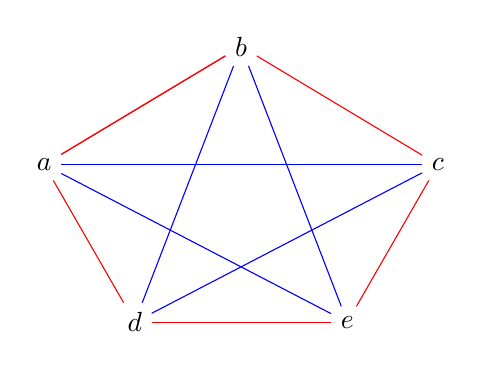
\begin{tikzpicture}
            \node (a) at (0,0) {$a$};
            \node (b) at (2.5,1.5) {$b$};
            \node (c) at (5,0) {$c$};
            \node (d) at (1.15,-2) {$d$};
            \node (e) at (3.85,-2) {$e$};
            \draw[red] (a) -- (b);
            \draw[blue] (a) -- (c);
            \draw[red] (a) -- (d);
            \draw[blue] (a) -- (e);
            \draw[red] (b) -- (a);
            \draw[red] (b) -- (c);
            \draw[blue] (b) -- (d);
            \draw[blue] (b) -- (e);
            \draw[blue] (c) -- (d);
            \draw[red] (c) -- (e);
            \draw[red] (d) -- (e);
        \end{tikzpicture}
    \end{center}

    Clearly, this does not have a red complete subgraph on $3$ vertices
    nor a blue complete subgraph on $3$ vertices.
}

\nt{
    No one knows what $R(5,5)$ is. It is expected that
    no one will ever know what $R(6,6)$ is.
}

\thm{}{
    $R(r,s)$ always exists. In fact,

    \begin{align*}
        R(r,s) \le R(r-1,s) + R(r,s-1)
    \end{align*}
}

\begin{subproof}
    This is done by double induction on $r,s \ge 1$. \\

    \subsubsection*{Base Case}

    \begin{align*}
        R(r,1) = R(1,s)= 1
    \end{align*}

    This is clearly true, because a complete graph with $1$ vertex is gaurunteed to have a
    subgraph on $1$ vertex that is blue or red. The color chosen is irrelevant because there are no edges
    so the color is implicit. \\

    Trivially the inequality (i.e. the base case holds true) holds because:

    \begin{align*}
         & R(r,1) \le R(r-1,1) + R(r,1-1) \iff 1 \le 1 + 0 \iff 1 \le 1 \\
         & R(1,s) \le R(1-1,s) + R(1,s-1) \iff 1 \le 0 + 1 \iff 1 \le 1
    \end{align*}

    \subsubsection*{Inductive Step}

    Suppose that $R(r-1,s)$ and $R(r,s-1)$ exist and consider the complete graph with
    $R(r-1,s) + R(r,s-1)$ vertices. Pick a vertex $v$. There are $R(r-1,s) + R(r,s-1) - 1$
    edges incident to $v$. Split the adjacent vertices $w$ into two classes, RED and BLUE,
    depending on if $(v,w)$ is a red or blue edge. Clearly,

    \begin{align*}
        R(r-1,s) + R(r,s-1) = |RED| + |BLUE| + 1
    \end{align*}

    The LHS represnts the total number of vertices in the original graph we constructed. The RHS is the
    decomposition of this graph based on an arbitrary vertex $v$ based on the adjacent edge
    colors. Because the graph is complete, RED and BLUE will contain every vertex in the original
    graph except the arbitrary vertex $v$ which is why we add $1$. Thus, I claim that one of the
    following must be true:

    \begin{align*}
        |RED|  & \ge R(r-1,s) \\
        |BLUE| & \ge R(r,s-1)
    \end{align*}

    Suppose not. That is suppose that both $|RED| < R(r-1,s)$ and $|BLUE| < R(r,s-1)$.
    Then, $|RED| + 1 \le R(r-1,s)$ and $|BLUE| + 1 \le R(r,s-1)$

    \begin{align*}
        |RED| + |BLUE| + 2 & \le R(r-1,s) + R(r,s-1) \\
        |RED| + |BLUE| + 1 & < R(r-1,s) + R(r,s-1)
    \end{align*}

    But this is a contradiction as $|RED| + |BLUE| + 1 = R(r-1,s) + R(r,s-1)$. So either
    $|RED| \ge R(r-1,s)$ or $|BLUE| \ge R(r,s-1)$ \\

    Without loss of generality, suppose that $|RED| = R(r-1,s)$. Then, the vertices
    in RED, must have a red $K_{r-1}$ or a blue $K_{s}$. If the former is true, then
    this $K_{r-1}$ with $v$ forms a $K_{r}$ within the original graph (as each vertex in
    RED was connected to $v$ with a red edge). Otherwise, the latter is true and thus the original
    graph contains a $K_{s}$. In either case, the original graph contains a $K_{r}$ or
    a $K_{s}$. Thus, not only does $R(r,s)$ exist but the inequality holds true as we
    either need one less vertices than what is in $R(r-1,s) + R(r,s-1)$ or we need
    to include the same number of vertices as $R(r-1,s) + R(r,s-1)$.

    \begin{align*}
        R(r,s) \le R(r-1,s) + R(r,s-1)
    \end{align*}
\end{subproof}

\setcounter{chapter}{4}

\chapter{The Binomial Coefficients}

\section{L10: Binomial coefficients and the binomial theorem I}

Recall the following two facts:

\begin{itemize}
    \item $\binom{n}{k} = \binom{n}{n-k}$
    \item $\binom{n}{k} = \binom{n-1}{k} + \binom{n-1}{k-1}$
\end{itemize}

\nt{
    One can think o Pascal's formula (the second fact) as the recursive definition the compute
    binomial coefficients with the following initial conditions:

    \begin{align*}
        \binom{n}{0} = \binom{n}{n} = 1
    \end{align*}
}

\subsubsection*{Properties of the Binomial Coefficients}

\begin{itemize}
    \item The row sums give powers of $2$
    \item The symmetry of the binomial coefficient.
    \item The number $\binom{n}{k}$ is the number of paths SW-NE "/" and NW-SE "$\backslash$" steps from
          $\binom{0}{0}$ to $(n,k)$.
\end{itemize}

\begin{subproof}
    Proof of third property: \\

    The only way to get to $\binom{n}{k}$ is to pass through $\binom{n-1}{k}$ or $\binom{n-1}{k-1}$.
    From here, we can apply induction and pascal's formula to show that this is true.
\end{subproof}

\qs{}{
    Write Pascal's triangle as follows:
    \begin{align*}
        \begin{matrix*}
            1 & & & & & \\
            1 & 1 & & & & \\
            1 & 2 & 1 & & & \\
            1 & 3 & 3 & 1 & & \\
            1 & 4 & 6 & 4 & 1 & \\
            1 & 5 & 10 & 10 & 5 & 1 \\
        \end{matrix*}
    \end{align*}

    Now consider the sums along SW to NE: $1, 1, 1+1, 1+2, 1+3+1, 1+4+3, \dots$ We've seen
    these numbers beore. What are they? (Can you give a proof?)
}

\sol{
    Clearly this sequence is $1, 1, 2, 3, 5, 8, \dots$. This is the Fibonacci sequence. \\

    The Fibonacci sequence is defined as:

    \begin{align*}
        a_n = a_{n-1} + a_{n-2}
    \end{align*}

    While this can be solved with recursion we can craft a combinatorial model to represent this
    situation. Consider the $n$-the Fibonacci number and a strip of length $n$. Imagine we are going
    to fill this strip with Rabbits (size $1$) and Cadillacs (size $2$). At a point $n$, we have two
    choices,

    \begin{enumerate}
        \item Place a Rabbit and lose one space
        \item Place a caddilac and lose two spaces
    \end{enumerate}

    Clearly, this is defined by the recurrence above. We can use a Rabbit and thus there are $a_{n-1}$
    ways to fill the strip or we can use a Cadillac and thus there are $a_{n-2}$ ways to fill the strip.
}

\dfn{The Binomial Theorem}{
    Let $n \in \mathbb{Z}_{> 0}$. Then,

    \begin{align*}
        (x+y)^n & = x^n + \binom{n}{1}x^{n-1}y + \binom{n}{2}x^{n-2}y^2 + \dots + \binom{n}{n-1}x y^{n-1} + y^n \\
                & = \sum_{k=0}^n \binom{n}{k} x^{n-k} y^k                                                       \\
    \end{align*}
}

\begin{subproof}
    Consider the expression $(x+y)^n$ exanded such that:

    \begin{align*}
        (x+y)^n = (x+y)(x+y)(x+y)\cdots
    \end{align*}

    Consider the process of FOIL to exapnd this expression. The term $x^iy^j$ The coefficient of this term
    is the number of ways to choose $i$ $x$s and $j$ $y$s where $i+j=n$ which is:

    \begin{align*}
        \binom{i + j}{i} & = \binom{n}{i}         \\
                         & = \binom{n}{n-i}       \\
                         & = \binom{i+j}{(i+j)-i} \\
                         & = \binom{i+j}{j}       \\
                         & = \binom{n}{j}
    \end{align*}
\end{subproof}

\subsubsection*{Binomial Identities}

\begin{itemize}
    \item $\binom{n}{0} + \binom{n}{1} + \cdots + \binom{n}{n} = 2^n$.

          \begin{subproof}
              Set $x = y = 1$ and apply binomial theorem.
          \end{subproof}

    \item $\binom{n}{0} - \binom{n}{1} + \binom{n}{2} - \cdots + (-1)^n \binom{n}{n} = 0$.

          \begin{subproof}
              Set $x = 1$ and $y=-1$. Apply Binomial Theorem.
          \end{subproof}

    \item $\binom{n}{0} + \binom{n}{2} + \cdots = \binom{n}{1} + \binom{n}{3} + \cdots$

          \begin{subproof}
              Use the previous property and move the negative coefficients to the RHS.
          \end{subproof}

    \item $\binom{n}{0} + \binom{n}{2} + \binom{n}{4} + \cdots = 2^{n-1} = \binom{n}{1} + \binom{n}{3} + \cdots$
          \begin{subproof}
              Using the first property, we know the total sum of the coefficients to be $2^n$. In each of these
              equations, we have removed half of the terms so the new sum is $\frac{2^n}{2} = 2^{n-1}$.
          \end{subproof}
\end{itemize}

\qs{}{
    Evaluate:

    \begin{align*}
        \binom{n}{0} - 2\binom{n}{1} + 3\binom{n}{2} + \cdots + (-1)^n(n + 1)\binom{n}{n}
    \end{align*}
}
\sol{

    \begin{subproof}
        Consider a simplified binomial theorem where $y=1$:

        \begin{align*}
            (x+1)^n = \sum_{i=0}^{n} \binom{n}{i}x^i
        \end{align*}

        By taking the derivative of both sides:

        \begin{align*}
            n(x+1)^{n-1} = \sum_{i=1}^{n} i \binom{n}{i} x^{i-1}
        \end{align*}

        Let $x=-1$.

        \begin{align*}
            0           & = \sum_{i=1}^n i \binom{n}{i} (-1)^{i-1}      \\
            (-1)\cdot 0 & = (-1) \sum_{i=1}^n i \binom{n}{i} (-1)^{i-1} \\
            0           & = \sum_{i=1}^n i \binom{n}{i} (-1)^{i}
        \end{align*}

        Lastly, we can add this with property $2$ above to obtain the desired result.
    \end{subproof}
}

\qs{}{
    Prove that the sequence of numbers in each row of Pascal's triangle is a power of 11. 
    I.e., $\{1,2,1\} \to 121=112$. For this you need to "carry over" numbers bigger than 9 to 
    the left. So for example $\{1,5,10,10,5,1\}$ is $161051=115$.
}
\sol{
    Consider the binomial expansion of $(1+x)^n$ and let $x=10$: 

    \begin{align*}
        (x+1)^n &= \sum_{i=0}^{n} \binom{n}{i}x^i \\ 
        11^n &= \sum_{i=0}^{n} \binom{n}{i}10^i \\
        11^n &= \binom{n}{0} + \binom{n}{1}10 + \binom{n}{2}100 + \cdots + \binom{n}{n}10^n
    \end{align*}
}

\qs{}{
    Give a combinatorial proof that the number of ways to select even sized 
    subsets equals the number of ways to select odd sized subsets (equals $2^{n-1}$).
}
\sol{
    We can encode a an even sized subset by recording which numbers from $1$ to $n-1$ 
    are being used. If this encoded subset is odd, then it can be inferred that 
    $n$ must have been used (since this is a encoding of an even sized subset). If 
    this encoded subset is even, then it can be inferred that $n$ was not used. Because 
    of this, the number of even subsets is simply the number of subsets that we can 
    create using elements of the set $\{1, 2, \dots, n-1\}$ which is $2^{n-1}$. The 
    same reasoning and connclusion applies to the odd sized subsets.
}

\section{L11: Binomial coefficients and the binomial theorem II}



\section{L12: Binomial coefficients and the binomial theorem III}

\subsection*{Applied and Abstract Context}

\subsubsection*{Applied}

Suppose that you're a designer of houses that you plan to put in a newly 
constructed neighbourhood. Each house is basically the same, but can be adorned with 
some of the following $n$ upgrades: 

\begin{itemize}
    \item Hard wood floors 
    \item Skylight
    \item Granite Countertops
    \item Stainless stell appliances
    \item $\dots$
\end{itemize}

\noindent
In order to be unique, you want to give each house a different set of options, BUT, 
no house A has upgrades that are a subset of another house B's upgrades (otherwise 
the owner of house A would be majorized by house B). By doing this, no two houses 
are comparable (one house may have hardwood floors, and other a sun roof). \\

\noindent
What is the maximum number of houses you can design under these conditions?

\subsubsection*{Abstract}

Consider the following poset (partially ordered set) for $S=\{x,y,z\}$: 

\begin{center}
    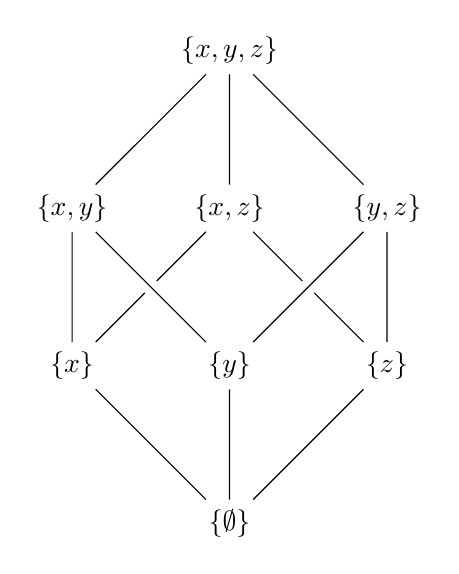
\begin{tikzpicture}
        \node (max) at (0,4) {$\{x,y,z\}$};
        \node (a) at (-2,2) {$\{x,y\}$};
        \node (b) at (0,2) {$\{x,z\}$};
        \node (c) at (2,2) {$\{y,z\}$};
        \node (d) at (-2,0) {$\{x\}$};
        \node (e) at (0,0) {$\{y\}$};
        \node (f) at (2,0) {$\{z\}$};
        \node (min) at (0,-2) {$\{\emptyset\}$};
        \draw (min) -- (d) -- (a) -- (max) -- (b) -- (f)
        (e) -- (min) -- (f) -- (c) -- (max)
        (d) -- (b);
        \draw[preaction={draw=white, -,line width=6pt}] (a) -- (e) -- (c);
    \end{tikzpicture}
\end{center}

\chapter{The Inclusion-Exclusion Principle and Applications}

\section{L13: The Inclusion-Exclusion principle and applications I}

\qs{}{
    How big is $A \cup B \cup C$?
}
\sol{
    \begin{align*}
        |A \cup B \cup C| = |A| + |B| + |C| - |A \cap B| - |A \cap C| - |B \cap C| + |A \cap B \cap C|
    \end{align*}

    If we just sum up the sizes of the sets, we are counting the
    elements in common between each of the sets twice. However,
    after we subtract out the number of elements in each intersection,
    we are excluding elements in commonb between all three sets.
}

\subsection*{}
This is the basis of the inclusion-exclusion principle.

\qs{}{
    How many elements are \textit{not} in $A, B,$ or $C$?
}
\sol{
    Let $S$ be the universal set.
    \begin{align*}
        |A^c \cap B^c \cap C^c| & = |S| - |A \cup B \cup C|                                                                          \\
                                & = |S| - \bigg ( |A| + |B| + |C| - |A \cap B| - |A \cap C| - |B \cap C| + |A \cap B \cap C| \bigg )
    \end{align*}
}

\ex{}{
    Find the number of integers between $1$ and $1000$ inclusive
    that are not divisible by $5$ and not divisible by $6$ and
    not divisible by $8$. \\

    Let

    \begin{itemize}
        \item $A_1$ be the subset of integers divisible by $5$,
        \item $A_2$ be the subset of integers divisible by $6$,
        \item $A_3$ be the subset of integers divisible by $8$.
    \end{itemize}

    Then we want to find $|A_1^c \cap A_2^c \cap A_3^c|$. \\

    \begin{align*}
        |A_1^c \cap A_2^c \cap A_3^c| & = |S| - |A_1 \cup A_2 \cup A_3|                                           \\
                                      & = |S| - \bigg ( |A_1| + |A_2| + |A_3| - |A_1 \cap A_2| - |A_1 \cap A_3| -
        |A_2 \cap A_3| + |A_1 \cap A_2 \cap A_3| \bigg )                                                          \\
    \end{align*}

    Obviously, $|S| = 1000$. To obtain the number of integers between $a$
    and $b$, where $b \geq a$, we can use the formula $\floor{\frac{b}{a}}$. \\

    \begin{align*}
        |A_1| & = \floor{\frac{1000}{5}} = 200 \\
        |A_2| & = \floor{\frac{1000}{6}} = 166 \\
        |A_3| & = \floor{\frac{1000}{8}} = 125
    \end{align*}

    Similarly,

    \begin{align*}
        |A_1 \cap A_2|          & = \floor{\frac{1000}{\lcm{5, 6}}} = \floor{\frac{1000}{30}} = 33    \\
        |A_1 \cap A_3|          & = \floor{\frac{1000}{\lcm{5, 8}}} = \floor{\frac{1000}{40}} = 25    \\
        |A_2 \cap A_3|          & = \floor{\frac{1000}{\lcm{6, 8}}} = \floor{\frac{1000}{24}} = 41    \\
        |A_1 \cap A_2 \cap A_3| & = \floor{\frac{1000}{\lcm{5, 6, 8}}} = \floor{\frac{1000}{120}} = 8
    \end{align*}

    Thus,

    \begin{align*}
        1000 - \bigg ( 200 + 166 + 125 - 33 - 25 - 41 + 8 \bigg ) & = 1000 - 200 - 166 - 125 + 33 + 25 + 41 - 8 \\
                                                                  & = 600
    \end{align*}
}

\qs{}{
    How many permutations of M,A,T,H,I,S,F,U,N are there where MATH,
    IS and FUN do not appear as consecutive letters?
}
\sol{
    Let

    \begin{itemize}
        \item $A_1$ be the set of permutations where MATH appears as consecutive letters,
        \item $A_2$ be the set of permutations where IS appears as consecutive letters,
        \item $A_3$ be the set of permutations where FUN appears as consecutive letters.
    \end{itemize}

    Then we want to find $|A_1^c \cap A_2^c \cap A_3^c|$. \\

    \begin{align*}
        |A_1^c \cap A_2^c \cap A_3^c| & = |S| - |A_1 \cup A_2 \cup A_3|                                                                                            \\
                                      & = |S| - \bigg ( |A_1| + |A_2| + |A_3| - |A_1 \cap A_2| - |A_1 \cap A_3| - |A_2 \cap A_3| + |A_1 \cap A_2 \cap A_3| \bigg ) \\
    \end{align*}

    Obviously, $|S| = 9!$. \\

    \begin{align*}
        |A_1| & = 6! \\
        |A_2| & = 8! \\
        |A_3| & = 7!
    \end{align*}

    Similarly,

    \begin{align*}
        |A_1 \cap A_2|          & = 5! \\
        |A_1 \cap A_3|          & = 4! \\
        |A_2 \cap A_3|          & = 6! \\
        |A_1 \cap A_2 \cap A_3| & = 3!
    \end{align*}

    Thus,

    \begin{align*}
        9! - \bigg ( 6! + 8! + 7! - 5! - 4! - 6! + 3! \bigg ) & = 9! - 6! - 8! - 7! + 5! + 4! + 6! - 3! \\
    \end{align*}
}

\thm{General Form of the Complementary Inclusion-Exclusion Principle}{
    \begin{align*}
        |A_1^c \cap \cdots & \cap A_m^c| = |S| - \sum |A_i| + \sum |A_i \cap A_j|                            \\
                           & - \sum |A_i \cap A_j \cap A_k| + \cdots + (-1)^{m+1} |A_1 \cap \cdots \cap A_m|
    \end{align*}
}

\begin{subproof}
    To begin, we can realize that the LHS counts the number of elements in $S$
    that are not in any of the $A_i$. \\

    For the RHS, Consider an arbitrary $s \in S$. There are two cases:

    \begin{itemize}
        \item Case 1. $x$ is not in any $A_i$.

              In this case, $x$ would contribute $1$ to the LHS and $1$ to
              RHS as it will not appear in any of the summations. Thus, this
              value will have no impact on the equality.

        \item Case 2. $x$ is in some $n > 0$ $A_i$ sets.

              Clearly, the contribution to the LHS is $0$. For the RHS,
              the contribution is

              \begin{align*}
                  1 + \sum_{k=1}^{n}(-1)^{k} \binom{n}{k}
              \end{align*}

              This is because we must count the number of ways to choose $k$
              sets from the $n$ sets that $x$ is in. \\

              By the binominal theorem, we have

              \begin{align*}
                  1 + \sum_{k=1}^{n}(-1)^{k} \binom{n}{k} & = \sum_{k=0}^{n} (1)^{n-k}(-1)^k\binom{n}{k} \\
                                                          & = (1 - 1)^n                                  \\
                                                          & = 0
              \end{align*}

    \end{itemize}

    In both cases, the equality holds. Thus, the LHS and RHS are equal.
\end{subproof}

\section{L14: The Inclusion-Exclusion principle and applications II: Derangements}

\subsection*{Introduction to Dearrangements}

\textbf{Question}: You all get up from your chairs, and randomly move to a different
chair. What's the probability that no one ends up sitting down
in the same chair? What if it were a class of $300$ students? \\

\nt{
    I find this definition a little hard to initially interpret. \\

    Derrangements can be thought of through the following example.
    Suppose a teacher is attempting to pass back a test to four students:
    $A, B, C, D$. There are obviously $4!$ ways to destribute the tests
    (i.e. there are $4!$ permutations of $A, B, C, D$). \\

    Dearrangements are the number of ways to distribute the tests such that
    no student gets their own test back. \\

    For example $A, C, D, B$ is not a dearragement because $A$ gets their
    own test back. However, $B, A, D, C$ is a dearrangement because no
    student gets their own test back. \\

    Our goal is count the number of dearrangements. \\
}

\qs{Abstract version of the original question} {
    Given a permutation $\pi \in S_n$, what is the probability
    that $\pi(i) \ne i$ for all $i$. What is the number of $D_n$
    for all such permutations?
}

\sol{Inclusion-Exclusion argument}{
    Let $A_i$ be the set of permutations where $\pi(i) = i$. \\

    Then we want to find $|A_1^c \cap A_2^c \cap \cdots \cap A_n^c|$. \\

    \begin{align*}
        |A_1^c \cap A_2^c \cap \cdots \cap A_n^c| & = |S_n| - |A_1 \cup A_2 \cup \cdots \cup A_n|                                                                    \\
                                                  & = |S_n| - \bigg ( |A_1| + |A_2| + \cdots + |A_n| - |A_1 \cap A_2| - |A_1 \cap A_3| - \cdots - |A_{n-1} \cap A_n| \\
                                                  & + |A_1 \cap A_2 \cap A_3| + \cdots + |A_{1} \cap \cdots \cap A_n| \bigg )                                        \\
    \end{align*}

    Clearly, there are $n!$ permutations in $S_n$. \\

    For each $0 \le i \le n$, there are $(n - 1)!$ permutations where $\pi(i) = i$.
    Thus there are $n(n - 1)!$ permutations where $\pi(i) = i$ for some $i$.
    So,

    \begin{align*}
        \sum_{i=1}^{n} |A_i| & = n(n - 1)! \\
                             & = n!
    \end{align*}

    For each $i,j$, there are $(n - 2)!$ permutations where $\pi(i) = i$ and $\pi(j) = j$.
    Thus there are $n(n - 1)(n - 2)!$ permutations where $\pi(i) = i$ and $\pi(j) = j$ for some $i$ and $j$.


    \begin{align*}
        \sum_{i,j}^{n} |A_i \cap A_j| & = \frac{n(n-1)(n-2)!}{2!} \\
                                      & = \frac{n!}{2}
    \end{align*}

    This makes sense because there are $n$ choices for $i$ and $n -1$
    choices for $j$ (since $i$ and $j$ cannot be the same). This leaves
    $(n-2)!$ ways to arrange the remaining $n - 2$ elements. However,
    $i$ and $j$ are indistinguishable, so we must divide by $2$ to account
    for this. \\

    Following this,

    \begin{align*}
        D_n & = n! - \frac{n!}{1!} + \frac{n!}{2!} - \frac{n!}{3!} + \cdots + (-1)^{n} \frac{n!}{n!} \\
            & = n!(1 - \frac{1}{1!} + \frac{1}{2!} - \frac{1}{3!} + \cdots + (-1)^{n} \frac{1}{n!})
    \end{align*}
}

\qs{}{
    What's the probability of picking a derangement as $n \to \infty$?
}
\sol{
    \begin{align*}
        \lim_{n \to \infty} \frac{D_n}{n!} & = \frac{1}{e}
    \end{align*}

    \nt{
        Just accept that this limit is true right now. Need to prove later.
    }
}

\qs{}{
    At a party, seven gentlemen check their hats.
    In how many ways can their hats be returned so that:

    \begin{itemize}
        \item no gentleman receives his own hat?
        \item at least one gentleman receives own hat?
        \item at least two gentlemen receive their own hat?
    \end{itemize}
}

\sol{part a}{

    This is simply the number of derangements for $n = 7$.

    \begin{align*}
        D_7 = 7!(1 - 1 + \frac{1}{2} - \frac{1}{3!} + \frac{1}{4!} - \frac{1}{5!} + \frac{1}{6!} - \frac{1}{7!})
    \end{align*}
}

\sol{part b}{

    This is just the total number of permutations - the number of
    derangements for 7 people. So,

    \begin{align*}
        7! - D_7
    \end{align*}
}

\sol{part c}{

    This is the number of ways that at least one person receives their own hat
    - the number of ways exactly one gentlement receives their own hat. \\

    \begin{align*}
        7! - D_7 - 7 \cdot D_6
    \end{align*}
}


\section{L15: The Inclusion-Exclusion principle and applications II}

\subsection*{Consider a problem we have seen before}
How many r-combinations are there of a multiset with $k$
distinct objects, each with infinite repetition number?

This is the same as the following question: Find the number
of integer solutions to

\begin{align*}
    x_1 + x_2 + \cdots + x_k = r
\end{align*}

subject to $x_i \ge 0$ or each $i$. We know the answer to this is

\begin{align*}
    \binom{r + k - 1}{r}
\end{align*}

Similarly, we have considered the problem where we assume instead
$x_i \ge a_i$.

\subsection*{New Problem}
Find the number of integer solutions to

\begin{align*}
    x_1 + x_2 + \cdots + x_k = r
\end{align*}

subject to $0 \le x_i \le a_i$ for each $i$. \\

\ex{How to solve this type of question}{

    Let $S$ be the set of solutions where we just have $x_i \ge 0$ and
    let $A_i$ be the set of solutions where $x_i > a_i$. Then we want
    to find $|A_1^c \cup A_2^c \cdots \cup A_m^c|$.

    \begin{align*}
        |A_1^c \cap \cdots & \cap A_m^c| = |S| - \sum |A_i| + \sum |A_i \cap A_j|                            \\
                           & - \sum |A_i \cap A_j \cap A_k| + \cdots + (-1)^{m+1} |A_1 \cap \cdots \cap A_m|
    \end{align*}
}

\qs{}{
    Find the number of integer solutions to

    \begin{align*}
        x_1 + x_2 + x_3 + x_4 = 18
    \end{align*}

    subject to $5 \ge x_1 \ge 1$, $4 \ge x_2 \ge -2$, $5 \ge x_3 \ge 0$, $9 \ge x_4 \ge 3$.
}
\sol{
    First, let us redefine the problem in terms of new variables with equal
    restrictions but started with $0$ as the lowest bound. \\

    The problem becomes:

    \begin{align*}
        y_1 + y_2 + y_3 + y_4 = 16
    \end{align*}

    subject to $4 \ge y_1 \ge 0$, $6 \ge y_2 \ge 0$, $5 \ge y_3 \ge 0$, $6 \ge y_4 \ge 0$. \\

    Now, let $S$ be the set of solutions where each $y_i \ge 0$. There are clearly,

    \begin{align*}
        \binom{16 + 4 - 1}{16} = \binom{19}{16}
    \end{align*}

    Now, we must solve each of the following intersections, however,
    we only need to consider the cases where the intersection is non-empty.
    This is obviously done by solving this like we have previously
    studied. Subtract $1 + $ the upper bound of each $y_i$ from the
    target value of the sums. And proceed to solve this question
    as a normal stars and bars problem. \\

    \begin{align*}
        |A_1| = \binom{11 + 4 - 1}{11} = \binom{14}{11}      \\
        |A_2| = \binom{9 + 4 - 1}{9} = \binom{12}{9}         \\
        |A_3| = \binom{10 + 4 - 1}{10} = \binom{13}{10}      \\
        |A_4| = \binom{9 + 4 - 1}{9} = \binom{12}{9}         \\
        |A_1 \cup A_2| = \binom{4 + 4 - 1}{4} = \binom{7}{4} \\
        |A_1 \cup A_3| = \binom{5 + 4 - 1}{5} = \binom{8}{5} \\
        |A_1 \cup A_4| = \binom{4 + 4 - 1}{4} = \binom{7}{4} \\
        |A_2 \cup A_3| = \binom{3 + 4 - 1}{3} = \binom{6}{3} \\
        |A_2 \cup A_4| = \binom{2 + 4 - 1}{2} = \binom{5}{2} \\
        |A_3 \cup A_4| = \binom{3 + 4 - 1}{3} = \binom{6}{3} \\
    \end{align*}

    So the final answer is

    \begin{align*}
         & = \binom{19}{16} - \Bigg ( \binom{14}{11} + \binom{12}{9} + \binom{13}{10} + \binom{12}{9}        \\
         & - \binom{7}{4} - \binom{8}{5} - \binom{7}{4} - \binom{6}{3} - \binom{5}{2} - \binom{6}{3} \Bigg ) \\
         & = 55
    \end{align*}

}

\section{L16: The Inclusion-Exclusion principle and
  applications IV: Another Forbidden Position Problem}

\qs{}{
    Eight people take a walk a walk in a line $$1,2,3,4,5,6,7,8$$ where
    1 precedes 2 who precedes 3 etc. How many ways are there to
    rearrange the people so that no one precedes the person he preceded
    before? \\

    In other words, count $w$ in $S_n$ that avoid the pairs
    $$1 2, 2 3, \dots, (n - 1) n$$
}

\sol{
    Let $S_n$ be the set of all permutations of $\{1, 2, \dots, n\}$.

    Let $A_i$ be the set of all permutations that contain the pair $i i+1$. \\

    Then we want to find
    \begin{align*}
        |S_n| - \Bigg ( \sum_{i=1}^{n} |A_i|     - \sum_{i,j=1}^{n} |A_i \cap A_j| + \cdots + (-1)^{n+1} |A_1 \cap \cdots \cap A_n| \Bigg )
    \end{align*}

    Clearly, $|S_n| = n!$ because there are $n!$ permutations. \\

    Now, we must solve each of the following intersections. Observe the following:

    \begin{align*}
        |A_{i_1} \cap A_{i_2} \cap \cdots \cap A_{i_k}| = \binom{n-1}{k} (n - k)!
    \end{align*}

    This is because we must think of constructing an algorithm that places the paired
    elements and then places the remaining elements. \\

    This algorithm is represented by the RHS of the above the equation. This
    is because there are only $n-1$ positions where we can place a "block",
    i.e., a pair of elements. Given $k$ blocks, there are $\binom{n-1}{k}$ ways to
    place them. Then, we must place the remaining $n-k$ elements
    which can be done in $(n-k)!$ ways given their distinct ordering \\

    Thus, this gives us the final form of the answer.

    \begin{align*}
        n! - \Bigg ( \binom{n - 1}{1}(n-1)! - \binom{n - 1}{2}(n-2)! + \cdots + (-1)^{n-1} \binom{n - 1}{n-1}(1)! \Bigg )
    \end{align*}
}

\thm{Non-attacking rook arragements}{
    The number of non-attacking rook arragements on an $n \times n$ board
    with forbidden positions is

    \begin{align*}
        n! - r_1(n-1)! + r_2(n-2)! - \cdots +(-1)^kr_k(n-k)! + \cdots + (-1)^n r_n
    \end{align*}

    Here $r_k$ is the number of ways to place $k$ rooks in the forbidden squares.
}

\begin{subproof}
    This is an application of the inclusion-exclusion principle. \\

    Let $A_i$ be the set of all placements where exactly one of the
    forbidden squares in row $i$ must be used. Consider the following
    arbitrary intersection of $A_i$s \\

    \begin{align*}
        \sum |A_{i_1} \cap A_{i_2} \cap \cdots \cap A_{i_k}|
    \end{align*}

    Note that the sum is over all selections of the $k$ subsets. \\

    This can be observed by constructing an algorithm that places the rooks
    in the forbidden squares and then places the remaining rooks. \\

    There are $r_k$ ways to place the rooks in the forbidden squares. Then,
    there are $n - k$ positions to place the remaining rooks, so there are
    $(n-k)!$ ways to place them. Thus,

    \begin{align*}
        \sum |A_{i_1} \cap A_{i_2} \cap \cdots \cap A_{i_k}| = r_k(n-k)!
    \end{align*}

    Substituting this is the inclusion-exclusion principle, we get
    the theorem.

\end{subproof}

\section{Practice Problems}

\chapter{Recurrence Relations and Generating Functions}
\section{L17: Some Number Sequences}

\ex{Example 1}{
    Consider a configuration of $n$ lines where every two lines
    have a point in common, but no three do. How many regions in the
    plane are there? Give a recurrence. \\

    $$
        a_n = a_{n-1} + n
    $$

    TODO: Give an explanation of why this is true.
}

\ex{Example 2}{
    Give a simple recurrence for dearragements. \\

    $$
        D_n = (n - 1)(D_{n-1} + D_{n-2})
    $$

    TODO: Give an explanation of why this is true. Need to review dearragements
    from previous lecture.
}

\subsubsection*{}
Consider the Fibonacci sequence $f_n = f_{n-1} + f_{n-2}$, where $f_0 = 0$ and $f_1 = 1$.

\dfn{The adjusted Fibonacci sequence: $\hat{F}_n$}{
    This is the number of 1,2 lists of size $n$. In other words,
    consider the number of ways a valet can park A cars (size $1$) and
    B cars (size $2$) in a parking lot of size $n$.

    \begin{equation*}
        \hat{F}_n = \begin{cases}
            1         & \text{if $n = 0$} \\
            f_{n + 1} & \text{otherwise}
        \end{cases}
    \end{equation*}
}

\qs{}{
    Prove
    $$
        \sum_{n=0}^{n} f_{i} = f_{n+2} - 1
    $$
}
\sol{
    \begin{subproof}
        We will prove this by induction on $n$. \\

        \textbf{Base case}: $n = 0$.
        $$
            \sum_{i=0}^{0} f_{i} = f_{0} = 0
        $$

        Similarly,
        $$
            f_{0+2} - 1 = f_{2} - 1 = 1 - 1 = 0
        $$

        So, the base case is true. \\

        \textbf{Inductive Hypothesis}: Assume that the following statement is true for $n = k$.

        $$
            \sum_{i=0}^{k} f_{i} = f_{k+2} - 1
        $$

        \textbf{Indcutive Step}: We will prove that the following statement is true for $n = k + 1$.

        $$
            \sum_{i=0}^{k+1} f_{i} = f_{k+1} + \sum_{i=0}^{k} f_{i} = f_{k+1} + f_{k+2} - 1 = f_{k+3} - 1
        $$

        Therefore, the statement is true for all $n$ by induction.
    \end{subproof}
}

\qs{}{
    Prove
    $$
        1 + \sum_{i=0}^{n} \hat{F}_i = \hat{F}_{n+2}
    $$
}
\sol{
    \begin{subproof}
        We will prove this by induction on $n$. \\

        \textbf{Base case}: $n = 0$.
        $$
            1 + \sum_{i=0}^{0} \hat{F}_i = 1 + \hat{F}_0 = 1 + 1 = 2
        $$
        Similarly,
        $$
            \hat{F}_{0+2} = \hat{F}_{2} = f_{2+1} = f_{3} = 2
        $$
        So, the base case is true. \\

        \textbf{Inductive Hypothesis}: Assume that the following statement is true for $n = k$.
        $$
            1 + \sum_{i=0}^{k} \hat{F}_i = \hat{F}_{k+2}
        $$

        \textbf{Inductive Step}: We will prove that the following statement is true for $n = k + 1$.
        \begin{align*}
            1 + \sum_{i=0}^{k+1} \hat{F}_i & = 1 + \hat{F}_{k+1} + \sum_{i=0}^{k} \hat{F}_i \\
                                           & = \hat{F}_{k+1} + \hat{F}_{k+2}                \\
                                           & = f_{k+2} + f_{k+3}                            \\
                                           & = f_{k+4}                                      \\
                                           & = \hat{F}_{k+3}                                \\
        \end{align*}

        Therefore, the statement is true for all $n$ by induction.
    \end{subproof}
}

\qs{}{
    Prove that $f_n$ is even if and only if $n$ is divisible by $3$.
}
\sol{
    \begin{subproof}
        Given that $f_0 = 0$, $f_1 = 1$, and $f_2 = 1$, we can see that
        at $n = 3$, $f_3 = 2$, which is even. \\

        This is because the only way to get an even number is to have
        the parity of the two numbers added togethed (odd + odd or even + even)
        be the same. So, $f_4$, must be odd, $f_5$ must be odd and
        $f_6$ must be even. \\

        Given the starting sequence of even, odd, odd. The following sequence
        must always be even, odd, odd, which repeats every $3$ numbers.

        Since the first $n = 0$ is the first number in the sequence, every $n$
        that is divisible by $3$ is even.
    \end{subproof}
}
\nt{
    Example problems for later \\

    Guess and prove by induction (you may replace the Fibonnaci
    number by the adjusted Fibonacci number if it helps you) \\

    \begin{itemize}
        \item $f_1 + f_3 + \cdots + f_{2n - 1} = ?$
        \item $f_0 + f_2 + \cdots + f_{2n} = ?$
        \item $f_0 - f_1 + f_2 - \cdots + (-1)^{n}f_n = ?$
        \item $(f_0)^2 + (f_1)^2 + \cdots + (f_n)^2 = ?$
    \end{itemize}
}

\subsubsection*{Obtaining an explicit formula for $f_n$ for linear recurrences}
\ex{}{
    Consider the Fibonacci sequence $f_n = f_{n-1} + f_{n-2}$, where $f_0 = 0$ and $f_1 = 1$.
    This can be rewritten as a linear recurrence as follows:
    $$
        f_n - f_{n-1} - f_{n-2} = 0
    $$

    We must solve the corresponding characterstic equation. Notice how the largest
    degree lines up with the "largest" case of the recurrence. \\

    $$
        x^2 - x - 1 = 0
    $$

    Let $q_1$ and $q_2$ be the roots of the characteristic equation. \\

    It is potentially relevant to note that the following is a solution space
    of the Fibonacci recurrence (but don't satisfy $f_0$ --
    the initial condition): \\

    \begin{equation*}
        \begin{cases}
            q_1^n - q_1^{n - 1} - q_1^{n - 2} = 0 \\
            q_2^n - q_2^{n - 1} - q_2^{n - 2} = 0 \\
        \end{cases}
    \end{equation*}

    The rest of this is based on an ansatz, i.e.
    we need to make an assumption at the answer and validate it later \\

    $$
        f_n = c_1q_1^n + c_2q_2^n,
    $$

    for \textit{some} $c_1, c_2 \in \mathbb{R}$. \\

    Using the initial conditions of $f_0 = 0$ and $f_1 = 1$,
    we can solve for $c_1$ and $c_2$.
}

\section{L18: Introduction to ordinary generating series}

\nt{
    Up until now, we have solved an instance combinatorial problem at a time.
    However, in some cases, solving a single combinatorial is too difficult.
    So, we solve all of the combinatorial problems at once.
}

\subsubsection*{}
Consider a sequence $$h_0, h_1, h_2, \dots, h_t, \dots$$ of natural numbers where
$h_t$ is the answer to some counting problem that depends on $t$. \\

We can create a generating series of the form:

$$
    g(x) = h_0 + h_1x + h_2x^2 + \cdots + h_tx^t + \cdots
$$

where $h_t = [x^t]g(x)$.

\nt{
    The notation $[x^t]g(x)$ is the coefficient of $x^t$ in the polynomial $g(x)$.
}

\clm{Compositions Generating Series}{}{
    $$
        g(x) = \Big ( \frac{1}{1 - x} \Big )^k
    $$
}

\ex{}{
    Fix $k$. Let \\

    $h_t = $ number of nonnegative integral solutions to
    $$
        e_1 + \cdots + e_k = t, e_i \in \mathbb{Z}_{\ge 0}
    $$

    We already know from stars and bars that

    $$
        h_t = \binom{t + k - 1}{k - 1}
    $$

    So obviously, the generating series can be written as

    $$
        g(x) = \sum_{t=0}^{\infty} \binom{t + k - 1}{k - 1}x^t
    $$

    \nt{
        This doesn't really tell us anything. We just combined some definitions
        and have a genearting series that is hard to utilize in any useful way.
    }

    Take our claim and expand it out with Taylor Series $k$ times:

    \begin{align*}
        g(x) & = \Big ( \frac{1}{1 - x} \Big )^k                                           \\
             & = (1 + x + x^2 + \cdots)(1 + x + x^2 + \cdots)(1 + x + x^2 + \cdots) \cdots \\
    \end{align*}

    We can see that the coefficient of $x^t$ is the number of ways to write $t$ as
    a sum of $k$ nonnegative integers. So,

    $$h_t = \binom{t + k - 1}{k - 1}$$

    This combinatorially proves the negative binomial theorem:

    $$
        g(x) = \Big ( \frac{1}{1 - x} \Big )^k
    $$
}

\subsubsection*{Remark}
If you knew that the negative binomial theorem was true,
you could use it to algebraically solve the composition problem after
choosing the correct generating series $g(x) = \Big ( \frac{1}{1 - x} \Big )^k$.

\qs{}{
    What is

    $$
        (1 + x + x^2 + x^3 + x^4 + x^5)( x + x^2)(1 + x + x^2 + x^3 + x^4)
    $$

    the generating series for?
}
\sol{
    The solutions to the equation

    $$
        e_1 + e_2 + e_3 = t
    $$

    where $0 \le e_1 \le 5, 1 \le e_2 \le 2, 0 \le e_3 \le 4$.
}

\qs{}{
    Suppose you have 1,5 and 25 cents coins available
    (infinite supply). Write down the generating series
    for the number of ways to make change for a dollar.
    How many ways are there?
}
\sol{

    The generating series for the number of ways to make change for an arbitrary amount of money is:

    $$
        g(x) = (1 + x + x^{1+1} + x^{1+1+1} + \cdots)(1 + x^{5} + x^{5+5} + x^{5+5+5} + \cdots)(1 + x^{25} + x^{25+25} + x^{25+25+25} + \cdots)
    $$

    This can be simplified as follows:

    \begin{align*}
        g(x) & = \Big ( \frac{1}{1 - x} \Big ) \Big ( \frac{1}{1 - x^{5}} \Big ) \Big ( \frac{1}{1 - x^{25}} \Big ) \\
             & = \frac{1}{(1 - x)(1 - x^{5})(1 - x^{25})}                                                           \\
    \end{align*}

    The answers is $[x^{100}]g(x)$.
}

\qs{Nonstandard Dice}{
    Compute the generating series for the result of rolling two standard dice. \\
    Now factor it, and interpret.
}
\sol{
    \begin{align*}
        g(x) & = (x + x^2 + x^3 + x^4 + x^5 + x^6)(x + x^2 + x^3 + x^4 + x^5 + x^6) \\
             & = (x + x^2 + x^3 + x^4 + x^5 + x^6)^2                                \\
             & = (1 + x)(1 + x)(x + x^3 + x^5)
    \end{align*}

    TODO: How does this factor like this?

    After factoring, we can see that this is the equivalent of
    flipping a coin twice and rolling two 1-3-5 dice.
}

\qs{}{
    Determine the generating series for partitions.
}
\sol{
    \begin{align*}
        g(x) & = (1 + x^{1} + x^{1+1} + x^{1+1+1} + \cdots)(1 + x^{2} + x^{2+2} + x^{2+2+2} + \cdots)(1 + x^{3} + x^{3+3} + x^{3+3+3} + \cdots) \cdots \\
             & = \Big ( \frac{1}{1 - x} \Big ) \Big ( \frac{1}{1 - x^{2}} \Big ) \Big ( \frac{1}{1 - x^{3}} \Big ) \cdots                              \\
             & = \prod_{i=1}^{\infty} \Big ( \frac{1}{1 - x^{i}} \Big )                                                                                \\
    \end{align*}
}

In words, this generating series is the product of compositions of just $1$'s, $2$'s, $3$'s, etc.

\dfn{Ordinary Generating Series}{
    Let a combinatorial problem be defined as $(S, \omega)$ with $S$ a set
    and $\omega: S \mapsto \mathbb{Z}_{\ge 0}$ The ordinary generating series is

    \begin{align*}
        g(x) = g_{(S, \omega)}(x) = \sum_{s \in S} x^{\omega(s)}
    \end{align*}
}

\thm{Addition Rule of Generating Series}{
    Suppose $S = A \cup B$ (disjoint union), where $(A, \omega_A)$
    and $(B, \omega_B)$ are combinatorial problems.
    Moreover $\omega|_A = \omega_A$ and $\omega|_B = \omega_B$.

    Then the ordinary generating series for $(S, \omega)$ is

    \begin{align*}
        g_{(S, \omega)}(x) & = g_{(A, \omega_A)}(x) + g_{(B, \omega_B)}(x)                     \\
                           & = \sum_{s \in A} x^{\omega_A(s)} + \sum_{s \in B} x^{\omega_B(s)} \\
                           & = \sum_{s \in S} x^{\omega(s)}
    \end{align*}
}

\nt{
    The notation $\omega|_A$ means the restriction of $\omega$ to $A$.
    In this case,

    $$
        \omega|_A = \{ \omega_A(s) \mid s \in A \}
    $$
}

\thm{Product rule of Generating Series}{
    Suppose $S = A \times B$ (cartesian product), where $(A, \omega_A)$
    and $(B, \omega_B)$ are combinatorial problems and

    \begin{align*}
        \omega(a, b) = \omega_A(a) + \omega_B(b)
    \end{align*}

    Then,

    \begin{align*}
        g_{(S, \omega)}(x) & = g_{(A, \omega_A)}(x)g_{(B, \omega_B)}(x)                      \\
                           & = \sum_{a \in A} x^{\omega_A(a)} \sum_{b \in B} x^{\omega_B(b)} \\
                           & = \sum_{a \in A} \sum_{b \in B} x^{\omega(a, b)}
    \end{align*}
}

\subsection*{What does it mean for two generating series to be equal?}

They are equal coefficient by coefficient.

\subsection*{Let $g(x)$ be the generating series for the number of partitions.
    What does it mean that $g(x)$ equals the infinite product:
}

\begin{align*}
    g(x) = \frac{1}{1 - x} \cdot \frac{1}{1 - x^{2}} \cdot \frac{1}{1 - x^{3}} \cdots
\end{align*}

It means that if we expand/solve enough terms of the RHS, the coefficient
of $x^t$ will stabalize (as in no more terms multiplied in will impact
the coefficient) and this coefficient will be the same as the coefficient
of $x^t$ in the LHS -- $g(x)$.

\subsection*{Convergence Issues}

Typically, with generating series, we only care about the coefficients and
not plugging in any specfic value into $x$. Because of this, we do not need
to worry about convergence. However, in some cases $g(x)$ is a polynomial
and in these cases, substitution is fine to perform.

\qs{Substituting into a generating series}{
    Let $S = \{$coins in your pokcet$\}$ and $\omega : S \mapsto \mathbb{Z}_{\ge 0}$
    be the obvious weight function on coins, i.e. $\omega$(nicket)$ = 5$. Is $g(x)$ is
    the corresponding generating series, what is $g(1)$? What is $g'(1)$?
}
\sol{
    $g(1)$ will be the number of coins in your pocket. This is trivially true
    because each term is $x$ to the power of an integer (with no coefficient),
    so $1$ raised to anything will be $1$ and so it is just the number of terms.
    More mathematically,

    \begin{align*}
        g(1) & = \sum_{s \in S} 1^{\omega(s)} \\
             & = \sum_{s \in S} 1             \\
             & = |S|
    \end{align*}

    $g'(1)$ will the amount of money you have. Based on the previous statement,
    we can see that the derivative of $g(x)$ is just the sum of the powers which
    represented the values of the coins in your pocket. More mathematically,
    \begin{align*}
        g'(1) = \sum_{s \in S} \omega(s)
    \end{align*}
}

\section{Practice Problems}

\qs{}{
    Find the coefficient of $x^{16}$ in $(x^2+x^3+\cdots)^5$.
}
\sol{
    This is the generating series for the following composition problem:

    \begin{align*}
        e_1 + e_2 + e_3 + e_4 + e_5 = 16
    \end{align*}

    where $e_1 \ge 2$, $e_2 \ge 2$, $e_3 \ge 2$, $e_4 \ge 2$, and $e_5 \ge 2$.

    This can be rewritten as:

    \begin{align*}
        e_1 + e_2 + e_3 + e_4 + e_5 = 6
    \end{align*}

    where each $e_i \ge 0$. Which represents the generating series:

    \begin{align*}
        g(x) & = (1 + x + x^2 + x^3 + x^4 + x^5 + \cdots)^5 \\
             & = \Big ( \frac{1}{1 - x} \Big )^5            \\
             & = (1-x)^{-5}                                 \\
    \end{align*}

    where we are solving for $[x^6]g(x) = \binom{5 + 6 - 1}{5 - 1} = \binom{10}{4}$.
}

\chapter{Special Counting Sequences}

\section{L19: Partition identities}

\dfn{Partition}{
    A \textit{partition} is a decreasing sequence of positive integers whose sum is $n$.
}

\ex{}{
    Consider $n = 5$. The partitions of $5$ are

    \begin{align*}
         & 5             \\
         & 4, 1          \\
         & 3, 2          \\
         & 3, 1, 1       \\
         & 2, 2, 1       \\
         & 2, 1, 1, 1    \\
         & 1, 1, 1, 1, 1
    \end{align*}

    However, this can also be represented in terms of the \textbf{Ferrers diagram}:

    Partitions $5$:

    \begin{align*}
         & \young(~~~~~)   \\
         & \young(~~~~,~)  \\
         & \young(~~~,~~)  \\
         & \young(~~~,~,~) \\
    \end{align*}

    \begin{align*}
         & \young(~~,~~,~)   \\
         & \young(~~,~,~,~)  \\
         & \young(~,~,~,~,~)
    \end{align*}
}

\ex{Theorem 8.3.1 from the textbook}{
    Use Ferrers diagrams to prove that the number of partitions of $n$
    in which the largest part is $r$ equals the number of partitions
    of $n-r$ in which no part is greater than $r$. \\

    Let $P$ be a partition for $n$. Remove the first part of $P$ which
    by definition is the largest part which has an arbitrary size $r$.
    This clearly yields a partition of $n-r$ in which no part is greater
    than $r$. This process is clearly a bijection and so the number of partitions
    of $n$ in which the largest part is $r$ equals the number of partitions
    of $n-r$ in which no part is greater than $r$. \\
}

\nt{
    This process for proving two partitions to be of equal size is important.
}

\subsection*{Generating Series , and partition identities}

Recall generating series for partition:

\begin{align*}
    g(x) = \prod_{k=1}^{\infty} \Big ( \frac{1}{1 - x^{k}} \Big )
\end{align*}

\qs{}{
    Write down the generating series for:

    \begin{enumerate}
        \item only odd parts
        \item no part repeated more than $m$ times
    \end{enumerate}
}
\sol{Only odd parts:}{
    \begin{align*}
        g(x) & = (1 + x^1 + x^{1+1} + x^{1+1+1} + \cdots) \cdot (1 + x^3 + x^{3+3} + x^{3+3+3} + \cdots) \cdot \cdots \\
             & = \prod_{k=1}^{\infty} \Big ( \frac{1}{1 - x^{2k-1}} \Big )
    \end{align*}
}

\sol{No part repeated more than $m$ times}{
    \begin{align*}
        g(x) & = (1 + x + x^{1 + 1} + \cdots + x^{m})(1 + x^{2} + x^{2 + 2} + \cdots + x^{2m})(1 + x^{3} + x^{3 + 3} + \cdots + x^{3m}) \cdots                \\
             & = (\frac{1}{1 - x} - \frac{x^m}{1 - x}) \cdot (\frac{1}{1 - x^2} - \frac{x^m}{1 - x^2}) \cdot (\frac{1}{1 - x^3} - \frac{x^m}{1 - x^3}) \cdots \\
             & = \prod_{k=1}^{\infty} \Big ( \frac{1}{1 - x^k} - \frac{x^m}{1 - x^k} \Big )                                                                   \\
             & = \prod_{k=1}^{\infty} \Big ( \frac{1 - x^m}{1 - x^k} \Big )
    \end{align*}
}

\subsection*{Terminology}

\dfn{Partition size}{
    The \textit{size} of a partition is the sum of its parts.
}

\dfn{Partition length}{
    The \textit{length} of a partition is the number of parts.
}

\qs{}{
    Write down a two variable generating series that counts partitions
    by both size and length, using say, a $q$ variable and a $z$ variable
    respectively. Hence the coefficient of $q^nz^l$ is the number of
    partitions of size $n$ and length $l$.
}
\sol{
    \begin{align*}
        g(q, z) & = \sum_{n=1}^{\infty} \sum_{l=1}^{\infty} P(n,l) \cdot q^{n}z^{l}    \\
                & = \prod_{k=0}^{\infty} (1 + zq^{k} + z^2q^{2k} + z^3q^{3k} + \cdots) \\
                & = \prod_{k=0}^{\infty} \Big ( \frac{1}{1 - zq^{k}} \Big )
    \end{align*}
}
\qs{}{
    Consider the identity:

    \begin{align*}
        \prod_{k=1}^{\infty} 1 + q^k = \prod_{k=1}^{\infty} \frac{1}{1 - q^{2k - 1}}
    \end{align*}

    \begin{itemize}
        \item Interpret both sides of the identity.
        \item Give an algabraic proof.
        \item Can you give a combinatorial proof?
    \end{itemize}
}
\sol{Interpret both sides of the identity}{
    \begin{itemize}
        \item LHS

              \begin{align*}
                  \prod_{k=1}^{\infty} 1 + q^k = (1 + q^1)(1 + q^2)(1 + q^3) \cdots
              \end{align*}

              This is clearly the number of partitions with distinct parts that
              are used at most one time.

        \item RHS

              This is clearly the generating series for partitions with only odd parts.
    \end{itemize}
}

\sol{Give an algebraic proof}{

    \begin{subproof}
        \begin{align*}
            \prod_{k=1}^{\infty} 1 + q^k & = \prod_{k=1}^{\infty} \frac{1-q^k}{1-q^k} (1 + q^k)                                   \\
                                         & = \prod_{k=1}^{\infty} \frac{1 - q^{2k}}{1 - q^k}                                      \\
                                         & = \prod_{k=1}^\infty \frac{ \frac{1}{1-q^k} }{ \frac{1}{1-q^{2k}} }                    \\
                                         & = \frac{ \prod_{k=1}^\infty \frac{1}{1-q^k} }{ \prod_{k=1}^\infty \frac{1}{1-q^{2k}} } \\
                                         & = \text { all even partitions divided out of all partitons }                           \\
                                         & = \prod_{k=1}^{\infty} \frac{1}{1 - q^{2k-1}}
        \end{align*}
    \end{subproof}
}

\sol{Give a combinatorial proof}{
    \begin{subproof}
        Fix $n$. Let $S$ be the set of all partitions of $n$ with only
        distinct parts. Clearly, the LHS represents the generating series that
        counts $S$. \\

        Construct a function $f$ from distinct parts to odd parts by dividing
        each even number by $2$ until every number is odd. This function is
        clearly well defined as it will only result in odd parts. This must
        be a bijection because the input to $f$ must have distinct parts so
        the number of odd parts created is dependent on the even numbers in
        the input so the output is unique. Lastly, this is clearly reversible
        by taking the largest subset of repeated odd numbers that is a power
        of $2$ and summing them. \\

        Thus, because we can decompose $S$ into the set of partitions with
        only odd parts through a bijective function and this decomposition
        is clearly counted by the RHS. Then, it is clear that the LHS and RHS
        equivalent.
    \end{subproof}
}

\section{L20: Partition identities (continued)}

\dfn{Partition Conjugate}{
    The \textit{conjugate} of a partition is the partition associated
    to the transpose of the Ferrers diagram. \\

    \begin{align*}
        \young(~~~~,~~,~)
    \end{align*}

    has a conjugate of

    \begin{align*}
        \young(~~~,~~,~,~)
    \end{align*}
}

\qs{}{
    Use conjugation to prove the following fact: the number of
    partitions of n with no part bigger than k equals the number
    of partitions of n with at most k parts. \\

    Determine the generating series for either of the kinds
    of partitions from the previous problem.
}
\sol{Using conjugation...}{
    \begin{subproof}
        This part is trivially true. If no part is bigger than $k$, then
        the first row in the Ferrers Diagram, which must be the largest row
        in the diagram, has at most $k$ parts.

        By taking the transpose of the first type of parition, we get a
        partition with at most $k$ parts as the number of parts will be
        dictated by the first row.

        Thus, the number of partitions of $n$ with no part bigger than $k$
        is the same as the number of partitions of $n$ with at most $k$ parts.
    \end{subproof}
}
\sol{Generating Series}{
    \begin{align*}
        g(x) = & (1 + x + x^{1+1} + \cdots + x^{k})           \\
               & (1 + x^2 + x^{2+2} + \cdots + x^{2k})        \\
               & (1 + x^3 + x^{3+3} + \cdots + x^{3k}) \cdots
    \end{align*}
    \begin{align*}
        g(x) & = \prod_{i=1}^{\infty} (1 + x^{i} + x^{2i} + \cdots + x^{ki})       \\
             & = \prod_{i=1}^{\infty} \Big ( \frac{1 - x^{ki+1}}{1 - x^{i}} \Big )
    \end{align*}
}

\dfn{Durfee Square}{
    A \textit{Durfee square} is the largest square that sits in the NW
    corner of the Ferrers diagram of a partition.
}

\qs{}{
    Show that every Ferrers shape uniquely decomposes into
    $(D_k, A_k, B_k)$ where $D_k$ is a Durfee square of size $k$,
    $A_k$ is the partition with at most $k$ parts, and $B_k$ is
    a partition with first part of size at most $k$.
}
\sol{
    Consider an arbitrary partition:

    \begin{align*}
        \young(~~~~,~~,~)
    \end{align*}

    This can obviously be decomoposed into the triple:

    \begin{align*}
        \Bigg ( \young(~~,~~) , \young(~~) , \young(~) \Bigg )
    \end{align*}

    There are a few cases to consider:

    \begin{itemize}
        \item First, this is unique. Clearly, this has to be unique
              because we are not changing any structure from the partition,
              but rather we are just decomposing it into a triple. So each
              partition must uniquely map to its own ordered triple. \\
        \item Second, $A_k$ is the partition with at most $k$ parts. $A_k$
              must have at most $k$ because the Durfee square is of size $k$. $A_k$
              cannot be largely than this because it would contradict either
              the definition of a partition or the definition of a Durfee square. \\
        \item Third, $B_k$ is the partition with first part of size at most $k$.
              This is true because if the first part of $B_k$ is larger than $k$, then
              this would contradict the definition of a Durfee square or a partition. \\
    \end{itemize}

    Thus, we have shown that every partition can be decomposed into a triple.
}

\dfn{Euler-Gauss Identity}{
    \begin{align*}
        \prod_{k=1}^{\infty} \frac{1}{1 - x^k} = 1 + \sum_{j=1}^{\infty} \frac{x^{j^2}}{\Big ( \prod_{t=1}^{j} 1 - x^t \Big )^2}
    \end{align*}
}

\dfn{Self-conjugate Partition}{
    A partition is \textit{self-conjugate} i its transpose shape is the same
    as its original shape (e.g., the partitions (4,1,1,1) and (3,2,1)
    are self-conjugate, but (3,2) is not).
}

\qs{}{
    Prove that the number of self conjugate partitions of $n$
    equals the number of partitions using only distinct odd parts.
    Then derive an identity.
}
\sol{
First, we must prove the number of self conjugate partitions of $n$
equals the number of partitions using only distinct odd parts. This
can be done by showing a weight preserving bijection between the
two sets. \\

\dfn{Weight-preserving function}{
    Define the following function:

    \begin{align*}
        f : (S, \omega) \mapsto (S', \omega')
    \end{align*}

    such that $\omega : S \mapsto \mathbb{Z}_{\ge 0}$
    and $\omega' : S' \mapsto \mathbb{Z}_{\ge 0}$ are weight functions.
    Then, $f$ is a weight-preserving function if and only if:

    \begin{align*}
        \omega(s) = \omega'(f(s)) \text{ for all } s \in S
    \end{align*}
}

And so, we can make the following claim

\clm{}{}{
    If $f : (S, \omega) \mapsto (S', \omega')$ is a weight-preserving
    and bijective  then,

    \begin{align*}
        g_{(S, \omega)}(x) = g_{(S', \omega')}(x) \in \mathbb{Z}[x]
    \end{align*}

    In other words, their generating functions are equal.
}

Now to define the actual bijection. Consider each row of the Ferrers
diagram of an arbitrary distinct odd partition. Each row can be
bent into a self-conjugate partition. By selecting the middle element,
which is gaurunteed to exist because the partition is odd, we can
place every square to the left below the middle element and leave
the other elements alone. Additionally, this is well defined as each
row is distinct. Thus, we have a weight preserving bijection
between the set of distinct odd partitions and the set
of self-conjugate partitions. \\

The generating function for the number of distinct odd partitions
is trivial and given by:

\begin{align*}
    g(x) = \prod_{i=1}^{\infty} 1 - x^{2i-1}
\end{align*}

as we only want to either select an odd number or not. \\

The generating function for the number of self-conjugate partitions
is more complicated. Consider an arbitrary self-conjugate partition
$\lambda$. We can decompose it into a triple $(D_k, A_k, B_k)$ through
the Durfee square decomposition. We can then apply a second weight-preserving
bijection and conjugate the second component of the triple which makes
$A_k = B_k$. Lastly, we can apply a third weight-preserving bijection
by compressing the triple into a tuple $(D_k, C_k)$ where $C_k$ is
$A_k$ merged left-to-right with $B_k$. \\

Consequently,

\begin{align*}
    C_k \in \bigcup_{j=0}^{\infty} D_j \times \text{Partitions}_{\text{even}_{\le j \text { tall}}} = U
\end{align*}

Clearly,

\begin{align*}
    g_{U}(x) & = \sum_{j=0}^{\infty} x^{j^2} \Big ( \prod_{t=1}^{j} \frac{1}{1 - x^{2t}} \Big ) \\
             & = \sum_{j=0}^{\infty} \frac{x^{j^2}}{\prod_{t=1}^{j} \frac{1}{1 - x^{2t}}}
\end{align*}

So,

\begin{align*}
    \prod_{k=1}^{\infty} 1 + x^{2k - 1} = \sum_{j=0}^{\infty} \frac{x^{j^2}}{\prod_{t=1}^{j} 1 - x^{2t}}
\end{align*}


\section{L21: Exponential generating series}

Given a number sequence $$h_0, h_1, h_2, \dots$$ consider
using the \textit{exponential} series:

\dfn{Exponential Generating Series}{
    \begin{align*}
        g_{\text{exp}}(x) = \sum_{i=0}^{\infty}h_i\frac{x^i}{i!}
    \end{align*}
}

\subsection*{Why do we care about using this?}

\subsubsection*{Reason A}
Ordinary generating series typically won't have any algabraic properties
that are useful such as factorization. However, exponential generating
may have these properties. \\

\ex{}{
    Fix a positive integer $n$. Let

    $P(n,k) = $ the number of $k$ permutations of an $n$ set. In other words,
    select $k$ elements from $n$ set where order matters. \\

    \qs{}{
        Compute the ordinary and exponential generating series for
        $P(n,0), P(n,1), \dots$.
    }


    \sol{
        Let's consider how a single $P(n,k)$ is constructed. There
        are $\binom{n}{k}$ ways to pick $k$ elements from $n$ set
        and $k!$ ways to order them. So,

        \begin{align*}
            P(n,k) & = \binom{n}{k}k!        \\
                   & = \frac{n!}{k!(n-k)!}k! \\
                   & = \frac{n!}{(n - k)!}
        \end{align*}

        Clearly the ordinary generating series is:

        \begin{align*}
            g(x) & = \sum_{i=0}^{\infty} P(n,i)x^i              \\
                 & = \sum_{i=0}^{\infty} \frac{n!}{(n - i)!}x^i \\
        \end{align*}

        Additionally, the exponential generating series is:

        \begin{align*}
            g_{\text{exp}}(x) & = \sum_{i=0}^{\infty} P(n,i)\frac{x^i}{i!}              \\
                              & = \sum_{i=0}^{\infty} \frac{n!}{(n - i)!}\frac{x^i}{i!} \\
                              & = \sum_{i=0}^{\infty} \binom{n}{i} x^i                  \\
                              & = (1 + x)^n
        \end{align*}

        \nt{
            Note how the exponential series simplifies as compared
            to the ordinary series.
        }
    }

    \qs{}{
        What is the exponential generating series for the sequence $1,1,1,\dots$?
    }

    \sol{
        \begin{align*}
            g_{\text{exp}}(x) & = 1 + x + \frac{x^2}{2!} + \frac{x^3}{3!} + \dots \\
                              & = \sum_{i=0}^{\infty} \frac{x^i}{i!}              \\
                              & = e^x
        \end{align*}
    }
}

\subsubsection*{Reason B}
Ordinary series only work well for \textit{unlabeled} combinatorial sets,
whereas exponential generating are better for \textit{labeled}
combinatorial sets. \\

\ex{}{
    Consider $38$ identical balls, how many ways are thre to group
    them together into 3 different bags? This is a composition
    problem, and is an unlabeled problem (since all balls are
    identical). This is a composition problem with a solution of
    $\binom{38 + 3 - 1}{3 - 1}$ \\

    Now consider 38 students in MATH 413. How many ways are there
    to group them into 3 different groups? This is a \textit{labeled}
    version of the problem. The answer to this is $3^{38}$ because there
    $3$ choices for each distint student.
}

\qs{}{
    What is $e^{ax}$, for a natural number $a$, the exponential
    generating series for?
}
\sol{
    We know that $e^x = \sum_{i=0}^{\infty} \frac{x^i}{i!}$, so

    \begin{align*}
        e^{ax} & = \sum_{i=0}^{\infty} \frac{(ax)^i}{i!} \\
               & = \sum_{i=0}^{\infty} \frac{x^i}{i!}a^i
    \end{align*}

    $a^i$ is the number of words of length $i$ that can be
    generated from an alphabet of size $a$. \\
}

\qs{}{
    Find the exponential generating series for the number of
    ways to place $r$ (distinct) people into three different
    rooms with at least one person in each room. Repeat the
    problem with the extra condition of an even number of people.
}
\sol{One person in each room}{
    \begin{align*}
        g_{\text{exp}}(x) = \Big ( x + \frac{x^2}{2!} + \frac{x^3}{3!} + \dots \Big )^3
    \end{align*}
}
\sol{Even Number of people and one person in each room}{
    \begin{align*}
        g_{\text{exp}}(x) = \Big ( \frac{x^2}{2!} + \frac{x^4}{4!} + \cdots \Big )^3
    \end{align*}
}

\qs{}{
    Now say $r=25$ in the above exercise. Compute the actual number
    of ways to place $25$ people in three rooms with at least one
    person in each room.
}
\sol{}{
We have already computed the generating series for one person
in each room above. This generating series can be simplified even
further as:

\begin{align*}
    g_{\text{exp}}(x) & = \Big ( x + \frac{x^2}{2!} + \frac{x^3}{3!} + \dots \Big )^3                \\
                      & = (e^x - 1)^3                                                                \\
                      & = \sum_{i=0}^{3} \binom{3}{i} (e^{x})^{3-i} (-1)^i                           \\
                      & = \binom{3}{0}e^{3x} - \binom{3}{1}e^{2x} + \binom{3}{2}e^{x} - \binom{3}{3} \\
                      & = e^{3x} - 3e^{2x} + 3e^{x} - 1
\end{align*}

Our desired answer is $[x^{25}]g_{\text{exp}}(x)$, so the answer is as follows:

\begin{align*}
    [x^{25}]g_{\text{exp}}(x) & = [x^{25}]e^{3x} - 3[x^{25}]e^{2x} + 3[x^{25}]e^{x} - [x^{25}] \\
                              & = 3^{25} - 3\cdot 2^{25} + 3\cdot 1^{25}                       \\
                              & = 3^{25} - 3 \cdot 2^{25} + 3
\end{align*}
}

\chapter{Homework}

\section{Homework 1}

\section{Homework 2}

\section{Homework 3}

\section{Homework 4}

\section{Homework 5}

\section{Homework 6}

\section{Homework 7}

\qs{}{
    Determine the number of integral solutions of the equation

    \begin{align*}
        x_1 + x_2 + x_3 + x_4 = 20
    \end{align*}

    that satisfy

    \begin{align*}
        1 \le x_1 \le 6, 0 \le x_2 \le 7, 4 \le x_3 \le 8, 2 \le x_4 \le 6
    \end{align*}
}
\sol{
    We first need to reformat the question with adjusted restrictions:

    \begin{align*}
         & y_1 + y_2 + y_3 + y_4 = 13                                         \\
         & 0 \le y_1 \le 5, 0 \le y_2 \le 7, 0 \le y_3 \le 4, 0 \le y_4 \le 4
    \end{align*}

    This can be solved using the inclusion-exclusion principle: \\

    Let $S$ be the set of all solutions to the above equations where
    each $y_i \ge 0$. By stars and bars,

    $$
        |S| = \binom{13 + 4 - 1}{13} = \binom{16}{13}
    $$

    Let $A_i$ be the set of all solutions such that $y_i \ge a_i$ where
    $a_i$ is the exclusive upper integral bound for $y_i$ (e.g. $y_1 \ge 6$) \\

    \begin{align*}
        |A_1| = \binom{7 + 4 - 1}{7} = \binom{10}{7}         \\
        |A_2| = \binom{5 + 4 - 1}{5} = \binom{8}{5}          \\
        |A_3| = \binom{8 + 4 - 1}{8} = \binom{11}{8}         \\
        |A_4| = \binom{8 + 4 - 1}{8} = \binom{11}{8}         \\
        |A_1 \cap A_2| = 0                                   \\
        |A_1 \cap A_3| = \binom{2 + 4 - 1}{2} = \binom{5}{2} \\
        |A_1 \cap A_4| = \binom{2 + 4 - 1}{2} = \binom{5}{2} \\
        |A_2 \cap A_3| = \binom{0 + 4 - 1}{0} = \binom{3}{0} \\
        |A_2 \cap A_4| = \binom{0 + 4 - 1}{0} = \binom{3}{0} \\
        |A_3 \cap A_4| = \binom{3 + 4 - 1}{3} = \binom{6}{3}
    \end{align*}

    Note that the intersection of any 3 sets will have no solution. \\

    Substituting this into the complementary form of the inclusion-exclusion
    principle, we get:

    \begin{align*}
        \binom{16}{13} - \Bigg ( & \binom{10}{7} + \binom{8}{5} + \binom{11}{8} + \binom{11}{8}                       \\
                                 & - \binom{5}{2} - \binom{5}{2} - \binom{3}{0} - \binom{3}{0} - \binom{6}{3} \Bigg ) \\
                                 & = 96
    \end{align*}
}

\qs{}{
    Determine the number of permutations of $\{1, 2, \dots, 9\}$ in
    which at least one odd integer is in its natural position.
}
\sol{
    This is an application of the inclusion-exclusion principle. \\

    Let $A_i$ be the set of all permutations such that $i$ is in its natural
    position. \\

    We must calculate $|A_1 \cup A_3 \cup A_5 \cup A_7 \cup A_9|$ for the inclusion-exclusion
    principle. \\

    For the sizes of each set individually, the size of each set
    must be $8!$ because there is one option for the position that
    must be in place and then we  must place the 8 remaining numbers.
    There are $\binom{5}{1}$ ways to pick the odd number in place. \\

    Following this pattern we can build the inclusion-exclusion principle
    as follows:

    \begin{align*}
         & = \binom{5}{1} 8! - \binom{5}{2}7! + \binom{5}{3} 6! - \binom{5}{4} 5! + \binom{5}{5}4! \\
         & = 157824
    \end{align*}
}

\qs{}{
    What is the number of ways to place six nonattacking rooks on
    the 6-by-6 boards with forbidden positions as shown?

    \begin{align*}
        \young(\times\times~~~~,\times\times~~~~,~~\times\times~~,~~\times\times~~,~~~~\times\times,~~~~\times\times)
    \end{align*}
}
\sol{
    This is an application of the inclusion-exclusion principle. \\

    Let $S_n$ be the set of all boards with nonattacking rooks on an $n \times n$ board.
    Clearly, there are $n!$ boards within $S_n$. This can be
    observed by constructing an algorithm to place one rook at a time. \\

    Let $A_i$ be the set of all boards with exactly 1 rook in the forbidden
    in row $i$. \\

    We must calculate $$|A_1^c \cap A_2^c \cap \cdots \cap A_n^c|$$

    Note that it is unecessary to consider each subset of $A_i$ individually,
    but rather we should consider the sum of the selected subsets. This gives
    the following identity

    \begin{align*}
        \sum |A_{i_1} \cap A_{i_2} \cap \cdots \cap A_{i_k}| = r_k (n - k)!
    \end{align*}

    where $r_k$ is the number of ways to place $k$ rooks in forbidden positions. \\

    Substituting this into the complementary form of the inclusion-exclusion
    principle, we get:

    \begin{align*}
         & 6! - (r_1(6 - 1)! - r_2(6 - 2)! + r_3(6 - 3)! - r_4(6 - 4)! + r_5(6 - 5)! - r_6(6 - 6)!) \\
         & = 6! - r_1(5!) + r_2(4!) - r_3(3!) + r_4(2!) - r_5(1!) + r_6(0!)                         \\
         & = 6! - r_1(5!) + r_2(4!) - r_3(3!) + r_4(2!) - r_5 + r_6
    \end{align*}

    All that remains is to calculate $r_1, r_2, \dots, r_6$. \\

    \begin{align*}
         & r_1 = 12                                                                                                                                         \\
         & r_2 = \binom{3}{1}\cdot (2)+ \binom{3}{2} (4\cdot 4) = 3 \cdot 2 + 3 \cdot 16 = 6 + 48 = 54                                                      \\
         & r_3 = \binom{3}{2} \binom{2}{1} \cdot (2 \cdot 4) + \binom{3}{3} (4 \cdot 4 \cdot 4) = 3\cdot 2 \cdot 2 \cdot 4 + 1\cdot 64 = 48+64= 112         \\
         & r_4 = \binom{3}{2} \binom{2}{1} \cdot 2 + \binom{3}{1} \cdot 2 \cdot 4 \cdot 4 = 3\cdot 2\cdot 2\cdot 2 + 3\cdot 2\cdot 4\cdot 4 = 12 + 96 = 108 \\
         & r_5 = \binom{3}{2} \binom{2}{1} \cdot 2 \cdot 4 = 48                                                                                             \\
         & r_6 = 2 \cdot 2 \cdot 2 = 8
    \end{align*}

    Substituting these values into the formula, we get:

    \begin{align*}
        6! - (12(5!) - 54(4!) + 112(3!) - 108(2!) + 48 - 8) = 80
    \end{align*}
}

\section{Homework 8}

\qs{}{
    How many ways are there to arrange the letters in INTELLIGENT
    with at least two pairs of consecutive identical letters? (For example
    ITTNELLGENI is an arrangement we want to count, since it has “TT”
    and “LL”.)
}
\sol{
    This is an application of the inclusion-exclusion principle. \\

    Let $A_i$ be the set of all arrangements with exactly $i$ pairs of consecutive
    identical letters. \\

    We must calculate $$|A_2 \cup A_3 \cup \cdots \cup A_5|$$

    For $A_2$, there are $\binom{5}{2}$ ways to choose the two pairs of consecutive
    identical letters. There are 7 remaining letters with 3 remaining pairs
    which can be arranged in $\frac{7!}{2!2!2!}$ ways. \\

    For $A_3$, there are $\binom{5}{3}$ ways to choose the three pairs of consecutive
    identical letters. There are 5 remaining letters with 2 remaining pairs
    which can be arranged in $\frac{5!}{2!2!}$ ways. However,
    we must consider that the previous calculation $A_2$ double counted
    elements of $A_3$ by the number of pairs that were chosen, which was
    $2$. We must multiply this in to account for this.  \\

    Following this pattern, we can see the final answer is

    \begin{align*}
        \binom{5}{2}\frac{9!}{(2!)^3} - 2\cdot \binom{5}{3}\frac{8!}{(2!)^2} + 3\cdot \binom{5}{4}\frac{7!}{(2!)} - 4\cdot \binom{5}{5}6!
    \end{align*}

    \nt{
        Could probably use better explanations on why we need to multiply
        by the number of pairs chosen in the previous calculation.
    }
}

\qs{}{
    Let $n$ be a positive integer and let $p_1, p_2, \dots, p_n$ be
    all of the different prime numbers that divide $n$. Consider the
    Euler function $\phi$ defined by

    \begin{align*}
        \phi(n) = \big | \{ k : 1 \le k \le n, \gcd{(k,n)} = 1 \} \big |
    \end{align*}

    Use the inclusion-exclusion principle to show that

    \begin{align*}
        \phi(n) = n \prod_{i=1}^{n} 1 - \frac{1}{p_i}
    \end{align*}
}

\qs{}{
    Prove that the Fibonacci sequence is the solution of the
    recurrence relation

    \begin{align*}
        a_n = 5a_{n-4} + 3a_{n-5}, (n \ge 5)
    \end{align*}

    where $a_0=0, a_1=1, a_2=1, a_3=2, a_4=3$. Then use this formula
    to show that the Fibonacci numbers satisfy the condition that
    $f_n$ is divisble by $5$ if and only if $n$ is divisible by $5$.
}

\qs{}{
    Let $h_n$ equal the number of different ways in which the
    squares of a $1 \times n$ chessboard can be colored, using the
    colors red, white, and blue so that no two squares that are
    colored red are adjacent. Find and verify a recurrence relation
    that $h_n$ satisfies. Then find a formula for $h_n$ (using the
    characteristic equation method).
}

\qs{}{
    The \textit{Lucas numbers} $l_0, l_1, l_2, \dots, l_n, \dots$
    are defined using the same recurrence relation defining the
    Fibonacci numbers, but with different intial conditions:

    \begin{align*}
        l_n = l_{n-1} + l_{n-2}, (n \ge 2) \quad l_0 = 2, l_1 = 1
    \end{align*}

    Prove that

    \begin{itemize}
        \item $l_n = f_{n-1} + f_{n+1} \text{ for } n \ge 1$
        \item $l_0^2 + l_1^2 + \cdots + l_n^2 = l_n l_{n+1} + 2 \text{ for } n \ge 0$
    \end{itemize}
}

\qs{}{
    Let $a_n$ equal  the number of ternary strings of length $n$ made
    up of $0$s, $1$s, and $2$s such that the substrings $00$, $01$, $10$,
    and $11$ never occur. Prove that

    \begin{align*}
        a_n = a_{n-1} + 2a_{n-2}
    \end{align*}

    for $n \ge 2$ with $a_0 = 1$ and $a_1=3$. Then find a formula for
    $a_n$.
}

\qs{}{
    A population grows as follows: in the current generation,
    each Canadian chooses one American for the next generation,
    and each American chooses one Canadian and one American for
    the next generation. Generation 0 consists of one Canadian.
    What is the size of generation $n$? (Here we assume all older
    generations leave when the new generation is chosen.)
}


\section{Homework 9}

\qs{}{
    Prove that the partition function $p(n)(=\text{number of partitions of } n)$
    satisfies $p(n+1) > p(n)$.
}
\sol{
    By the definition of a partition, we know there are $p(n)$ sequences of decreasing
    positive integers that sum to $n$. \\

    For each sequence, we can append a $1$ to the end to construct a new sequence,
    which will still be decreasing and sum to $n+1$. Therefore, we know that $p(n+1)$
    is \textit{at least} $p(n)$. \\

    Additionally, we can construct a new partition of the sequence $\{n+1, 0, 0, \dots\}$.
    This will be a partition of $n+1$ trivially. Additionally, this partition cannot
    be a partition of any integer less than $n+1$ as the sum is above $n$. Since,
    this partition is not in $n$, we know that $p(n+1) > p(n)$.
}

\qs{}{
    For each integer $n > 2$ determine a self-conjugate partitoin of $n$
    that has at least two parts.
}
\sol{
    There are two cases to consider:

    \begin{itemize}
        \item $n$ is odd \\

              We can construct the follwing partition of $n$:

              \begin{align*}
                  \{\frac{n-1}{2} + 1, 1_1, 1_2, \dots, 1_{\frac{n-1}{2}}\}
              \end{align*}

              where there are $\frac{n-1}{2}$ $1$s. This is self-conjugate as it will create
              Ferrer Diagrams of the form:

              \begin{align*}
                  \young(~~~~,~,~,~)
              \end{align*}

              Since $n > 2$, we know that there are at least two parts. At $n=3$,
              $\frac{n-1}{2} + 1 = 2$ and $\frac{n-1}{2}=1$. So the partition is $\{2,1\}$. \\

              This is trivially bijective because $\frac{n-1}{2}$ is bijective.

        \item $n$ is even \\

              We know that $n-1$ is odd. So we can construct a sel-conjugate partition for $n-1$
              and then modify the generated sequence by changing one of the appended $1$s to a $2$.

              This generates Ferrer Diagrams of the form:

              \begin{align*}
                  \young(~~~~,~~,~,~)
              \end{align*}

              We have shown in the odd case that this is a bijection and partition,
              so we know that this is a self-conjugate partition of $n$ because adding
              $1$ to one of the parts is still a bijective action.
    \end{itemize}
}

\qs{}{
    Prove that the number of partitions of $n$ in which no part appears
    exactly once is equal to the number of partitions of $n$ with no
    parts congruent to $1$ or $5 \pmod{6}$.
}

\qs{}{
    Do part (c) of the last in class exercise of Lecture 19.
    That is, give a bijective proof that the number of partitions
    of $N$ using distinct parts equals the number of partitions of
    $N$ using only odd parts. (Hint: Consider the multiplicity $m_p$
    of each part $p$ occuring in partitions of the second type.
    Now look at the unique expansion of $m$ as powers of $2$ and
    distribute.)
}
\sol{
    Consider an arbitrary partition $P$ that only uses odd parts for $N$:

    \begin{align*}
        N = o_1 + o_2 + \cdots + o_k
    \end{align*}

    Group each odd number to obtain its multiplicity $m_p$ (e.g. 1 + 1 + 1 = 3(1)):

    \begin{align*}
        N = m_1 (o_1) + m_2 (o_2) + \cdots + m_k (o_k)
    \end{align*}

    Consider the unique expansion of $m_p$ as powers of $2$:

    \begin{align*}
        m_p = 2^0 + 2^1 + \cdots + 2^r
    \end{align*}

    Distribute each $o_i$ across the expansion of $m_p$:

    \begin{align*}
         & = (2^0  + 2^1 + \cdots + 2^{r_1}) o_1 + (2^0  + 2^1 + \cdots + 2^{r_2}) o_2 + \cdots + (2^0  + 2^1 + \cdots + 2^{r_k}) o_k                                                              \\
         & = 2^0 (o_{\alpha_1} + o_{\alpha_2} + \cdots + o_{\alpha_x}) + 2^1 (o_{\beta_1} + o_{\beta_2} + \cdots + o_{n_2}) + \cdots + 2^{r} (o_{\gamma_y} + o_{\gamma_2} + \cdots + o_{\gamma_z}) \\
    \end{align*}

    Let $a_i$ be the sum of the $o_i$s that correspond to the $2^i$ term:

    \begin{align*}
         & = 2^0 a_0 + 2^1 a_1 + \cdots + 2^{r} a_r
    \end{align*}

    We know that each of these terms must be unique as each power of $2$ is unique in this sequence.

    Thus, we have constructed a bijection between the partitions of $N$ using only odd parts
    and the partitions of $N$ using distinct parts.
}

\section{Homework 10}

\chapter{Midterms}

\section{Midterm 1}

\subsection{Practice Problems}

\subsection{Solutions}

\subsection{Exam}

\subsection{Exam Solutions}

\section{Midterm 2}

\subsection{Practice Problems}

\subsection{Solutions}

\subsection{Exam}

\subsection{Exam Solutions}

\section{Midterm 3}

\subsection{Practice Problems}

\qs{}{
    Find a recurrence relation for the number of different ways to hand
    out a piece of chewing gum (worth $1$ cent) or a candy bar (worth $10$
    cents) or a donut (worth $20$ cents), one item a day, until n cents worth
    of food has been given away. Don’t worry about the initial condition.
}
\sol{
    Let $f(n)$ be the number of ways to hand out a piece of chewing gum,
    a candy bar, or a donut with $n$ cents. At any moment with $n$ cents,
    we can either give a piece of gum, a candy bar, or a donut. This gives

    \begin{align*}
        f(n) = f(n-1) + f(n-10) + f(n-20)
    \end{align*}
}

\qs{}{
    By using generating series, determine the number of integer solutions
    to the composition problem

    \begin{align*}
        e_1 + e_2 + e_3 = 22
    \end{align*}

    subject to $3 \le e_1 \le 8$, $6 \le e_2 \le 10$, and $2 \le e_3 \le 7$.
}
\sol{
    Clearly this can be solved by the following generating series:

    \begin{align*}
        g_1(x) = (x^3+x^4+x^5+x^6+x^7+x^8) (x^6+x^7+x^8+x^9+x^{10}) (x^2+x^3+x^4+x^5+x^6+x^7)
    \end{align*}

    where the solution is $[x^22] g(x)$. However, this is difficult to extract
    a coefficient from. Instead, rewrite the problem in terms of new variables:

    \begin{align*}
        e_1 + e_2 + e_3 = 11
    \end{align*}

    where $0 \le e_1 \le 5$, $0 \le e_2 \le 4$, and $0 \le e_3 \le 5$.
    The generating series now becomes:

    \begin{align*}
        g_2(x) = (1 + x + x^2 + x^3 + x^4 + x^5) (1 + x + x^2 + x^3 + x^4) (1 + x + x^2 + x^3 + x^4 + x^5)
    \end{align*}

    where we are solving for $[x^{11}] g_2(x)$. This generating series can be simplified as follows:

    \begin{align*}
        g_2(x) & = (1 + x + x^2 + x^3 + x^4 + x^5) (1 + x + x^2 + x^3 + x^4) (1 + x + x^2 + x^3 + x^4 + x^5) \\
               & = (\frac{1 - x^{6}}{1 - x}) (\frac{1 - x^5}{1 - x}) (\frac{1 - x^6}{1 - x})                 \\
               & = \frac{(1 - x^{6}) (1 - x^5) (1 - x^6)}{(1 - x) (1 - x) (1 - x)}                           \\
               & = \frac{(1 - x^{6}) (1 - x^5) (1 - x^6)}{(1 - x)^3}                                         \\
               & = (1 - x^{6}) (1 - x^5) (1 - x^6) (1-x)^{-3}                                                \\
               & = (1 - x^{5} - x^{6} + x^{11})(1-x^{6}) (1-x)^{-3}                                          \\
               & = (1 - x^{5} - x^{6} + x^{11} - x^{6} + x^{11} + x^{12} - x^{17}) (1-x)^{-3}                \\
               & = (1 - x^{5} - 2x^{6} + 2x^{11} + x^{12} - x^{17}) (1-x)^{-3}                               \\
    \end{align*}

    The target solution is $[x^{11}] g_2(x)$. Using negative binomial theorem,
    we can find the coefficient of $x^{11}$ as follows:

    Reminder that negative binomial theorem is:

    \begin{align*}
        (1 - x)^{-n} = \sum_{k=0}^{\infty} \binom{n+k-1}{k} x^k
    \end{align*}

    \begin{align*}
        [x^{11}]g_2(x) & = [x^{11}]((1 - x^{5} - 2x^{6} + 2x^{11} + x^{12} - x^{17}) (1-x)^{-3})                                                                                         \\
                       & = [x^{11}] \Big ( (1-x)^{-3} - x^{5} (1-x)^{-3} - 2x^{6}(1-x)^{-3} + 2x^{11}(1-x)^{-3} + x^{12}(1-x)^{-3} - x^{17}(1-x)^{-3} \Big )                             \\
                       & = [x^{11}](1-x)^{-3} - [x^{11}]x^{5} (1-x)^{-3} + [x^{11}] 2x^{6}(1-x)^{-3} + [x^{11}]2x^{{11}}(1-x)^{-3} + [x^{11}]x^{12}(1-x)^{-3} - [x^{11}]x^{17}(1-x)^{-3} \\
                       & = [x^{11}](1-x)^{-3} - [x^6](1-x)^{-3} - 2 [x^{5}] (1-x)^{-3} + 2[x^0](1-x)^{-3} + [x^{-1}](1-x)^{-3} - [x^{-6}](1-x)^{-3}                                      \\
                       & = \binom{3+11-1}{3-1} - \binom{3+6-1}{3-1} - 2 \binom{3+5-1}{3-1} + 2 \binom{3+0-1}{3-1} + 0 + 0                                                                \\
                       & = \binom{13}{2} - \binom{8}{2} - 2 \binom{7}{2} + 2 \binom{2}{2}
    \end{align*}
}

\qs{}{
    Prove that the number of partitions where no part appears more
    than two times equals the number of partitions where no part is a
    multiple of three. (Hint: write down the generating series for the former
    type of partition and algebraically manipulate to get to the generating
    series for the latter type.)
}
\sol{
    Number of partitions of $n$ where no part appears more than two times:

    \begin{align*}
        \prod_{i=1}^{\infty} (1 + x^i + x^{2i})
    \end{align*}

    Number of partitions of $n$ where no part is a multiple of three:

    \begin{align*}
        \frac{
            \prod_{i=1}^{\infty} \frac{1}{1 - x^i}
        }{
            \prod_{i=1}^{\infty} \frac{1}{1 - x^{3i}}
        } & = \prod_{i=1}^{\infty} \frac{ \frac{1}{1 - x^i} }{ \frac{1}{1 - x^{3i}} } \\
          & = \prod_{i=1}^{\infty} \frac{1 - x^{3i}}{1 - x^i}
    \end{align*}

    Algabraic proof:

    \begin{subproof}
        \begin{align*}
            \prod_{i=1}^{\infty} (1 + x^i + x^{2i}) & = \prod_{i=1}^{\infty} \frac{(1+x^i+x^{2i})(1-x^i)}{1-x^i}                \\
                                                    & = \prod_{i=1}^{\infty} \frac{1+x^i+x^{2i} - x^i - x^{2i} - x^{3i}}{1-x^i} \\
                                                    & = \prod_{i=1}^{\infty} \frac{1 - x^{3i}}{1-x^i}                           \\
        \end{align*}
    \end{subproof}
}

\qs{}{
    Determine the number of permutations of $\{1, 2, 3, 4, 5, 6, 7, 8\}$ in
    which no even integer is in its natural position. For example, $43258176$
    is good, but $42358176$ is bad because of the position of the 2.
}
\sol{
    This is an application of inclusion-exclusion principle. \\

    Let $S$ be the set of all permutations of $\{1, 2, 3, 4, 5, 6, 7, 8\}$. Clearly,
    $|S| = 8!$. \\

    Let $A_i$ be the subset of permutations in $S$ where $i$ is in its natural position.
    We are looking to calculate the following by the complementary form of the
    inclusion-exclusion principle:

    \begin{align*}
        |A_2^c \cap A_4^c \cap A_6^c \cap A_8^c| = |S| - \sum |A_i| + \sum |A_i \cap A_j| - \sum |A_i \cap A_j \cap A_k| + |A_2 \cap A_4 \cap A_6 \cap A_8| \\
    \end{align*}

    Each sum can be calculated as follows:

    \begin{align*}
        \sum |A_{i_1} \cap A_{i_2} \cdots A_{i_k}| & = \binom{4}{k}(8-k)! \\
    \end{align*}

    This is because there are $4$ ways to choose the even numbers that are fixed.
    For each of these choices, there are $8-k$ ways to choose the remaining numbers. \\

    So, we have:

    \begin{align*}
        8! - \binom{4}{1}7! + \binom{4}{2} 6! - \binom{4}{3} 5! + \binom{4}{4} 4!
    \end{align*}
}

\qs{}{
    Define what it means for a pair $(S, \omega)$ means to be combinatorial
    problem. Define generating series in these terms. State and prove the
    product lemma. (As usual, on the test I might ask a \textbf{very precise}
    question about these proofs (or any proof) so you must be able to
    understand each line and symbol used in the argument.)
}

\subsection{Solutions}

\subsection{Exam}

\subsection{Exam Solutions}

}

\end{document}